% !TEX root = Nies_Lukas_BSc_Thesis_SiPM.tex

%Use letters for appendix referencing
%\renewcommand\thefigure{\thesection.\arabic{figure}} 

\chapter{Figures}

%\setcounter{figure}{0}    

\begin{figure}[H]
	\centering
	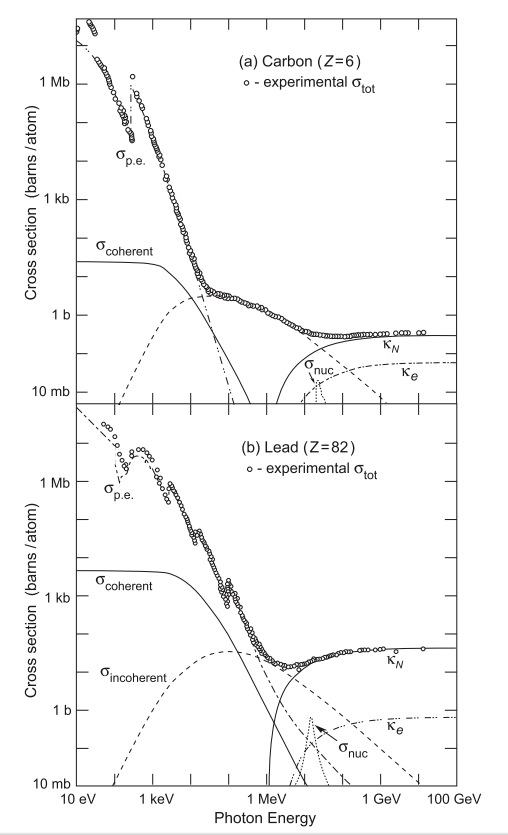
\includegraphics[width=0.65\textwidth]{./graphics/ch1/photo_absorption_cross_sections.png}
	\caption[Interaction of phtonos with matter (detailed)]{Energy dependence of the cross-section of photons in carbon and lead \cite{wermes}.}    
	\label{ap:A:photons_detailed}
\end{figure}

\newpage

\begin{figure}[t]
	\centering
	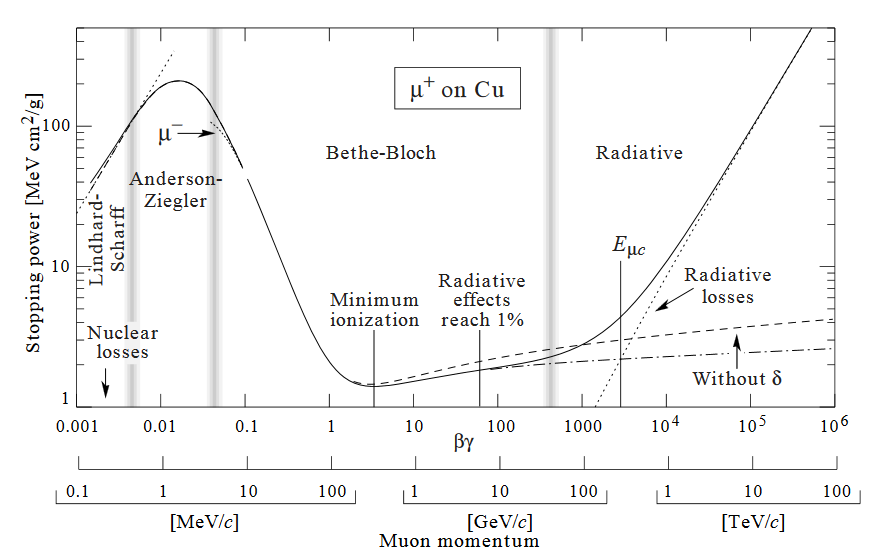
\includegraphics[width=0.85\textwidth]{./graphics/ch1/bethe_bloch_detailed.png}
	\caption[Stopping power for a wide energy range]{Stopping power for a wide energy range \cite{PDG}. The \textit{Bethe-Bloch} region is shown for $0.1<\beta\gamma<1000$.}    
	\label{ap:A:bethe_bloch_detailed}
\end{figure}

\newpage

\begin{figure}[t]
	\centering
	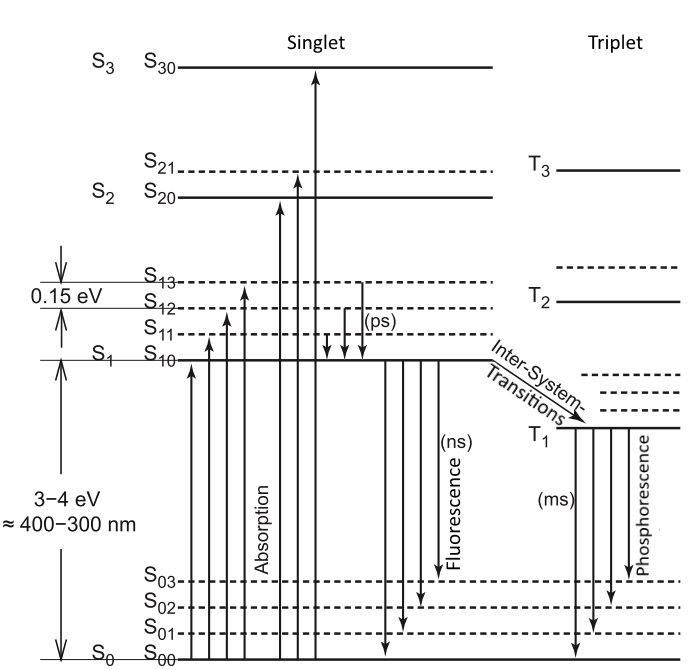
\includegraphics[width=0.85\textwidth]{./graphics/ch2/jablonski.png}
	\caption[Jablonski-Diagram]{Jablonski-Diagram for singlet and triplet states of $\pi$-electrons of a organic scintillator \cite{wermes}.}    
	\label{ap:A:jablonski}
\end{figure}

\chapter{Fits, Plots and data processing}

\section{IV-curves}

First, the region before breakdown has been fitted with a first order polynomial 
\begin{align*}
I(V)=m\cdot V+I_0
\end{align*} 
to find the offset $I_0$. This has then been substracted from the data to grant more precision when plotting $I$ in log scale. Now two polynomial functions have been used to determine the intersection of the point of breakdown
\begin{align*}
\log(I(V))&=m\cdot V+I_{0} & \log(I(V))&=A\cdot V^2+B\cdot V+C.
\end{align*}
By comparing both equations and solving V, one retrieves 
\begin{align*}
m\cdot V+I_{0} &= A\cdot V^2+B\cdot V+C \\
\Rightarrow V_{\pm} &= -\frac{B-m}{2A}\pm \sqrt{\left(\frac{B-m}{2A}\right)^2-\frac{C-I_0}{A}}, 
\end{align*}
where $V_\pm$ is the solution of this equation. The error $\Delta V$ has been calculated via error propagation of the fit errors:
\begin{align*}
\Delta V_\pm=\arrowvert\dv{V_\pm}{m}\arrowvert\Delta m+\arrowvert\dv{V_\pm}{I_0}\arrowvert\Delta I_0+\arrowvert\dv{V_\pm}{A}\arrowvert\Delta A+\arrowvert\dv{V_\pm}{B}\arrowvert\Delta B+\arrowvert\dv{V_\pm}{C}\arrowvert\Delta 
C.
\end{align*}
The fits can be found in figures \ref{ap:B:breakdown_fits_single} and \ref{ap:B:breakdown_fits_hybrid}.

\newpage

\begin{figure}[H]
	\subfloat[(s)-configuration $\SI{25}{\degreeCelsius}$] {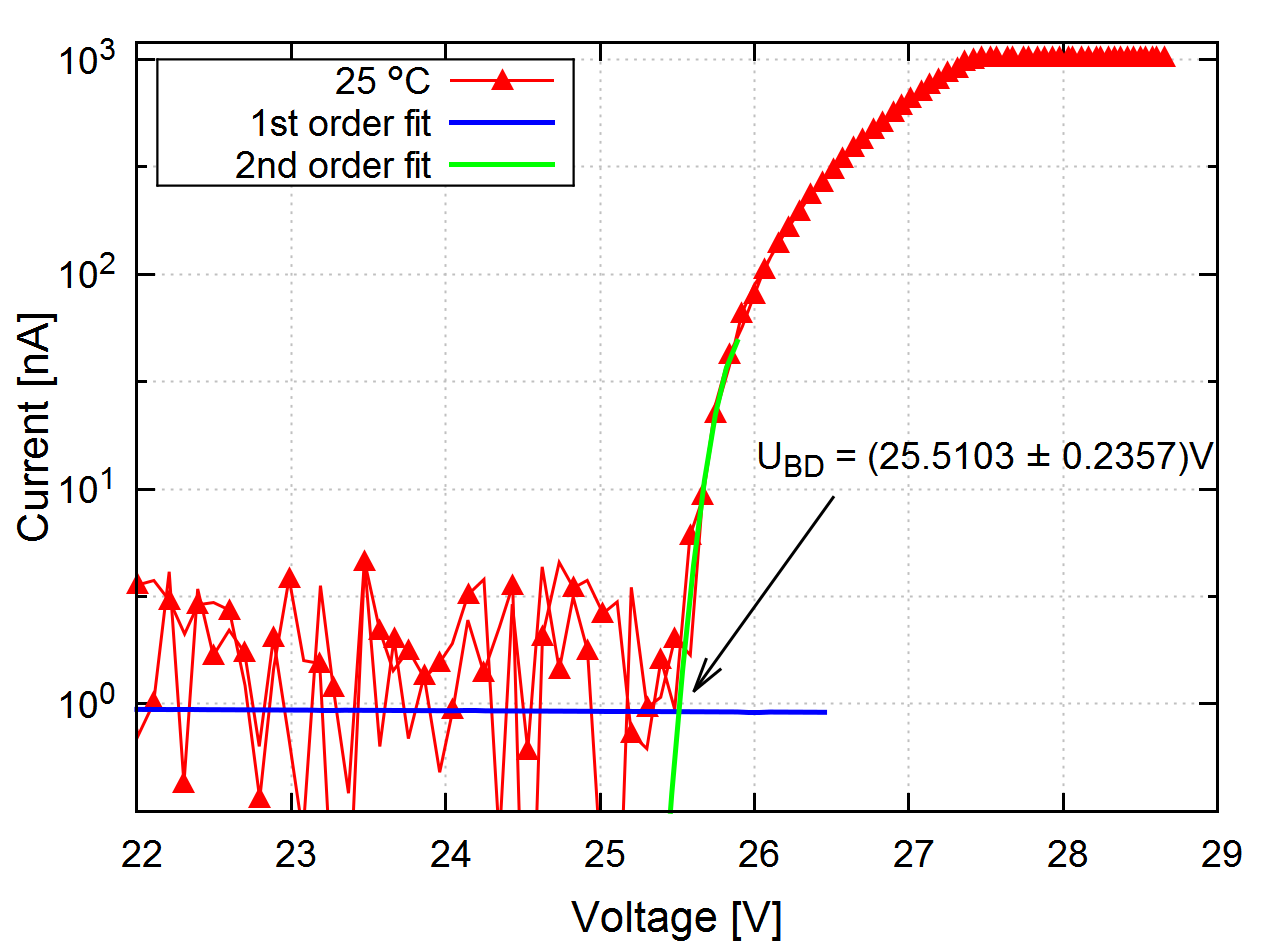
\includegraphics[width=0.49\textwidth]{./plots/iu_curve/1x1n2_bd_25.png}}
	\hfill
	\subfloat[(s)-configuration $\SI{20}{\degreeCelsius}$] {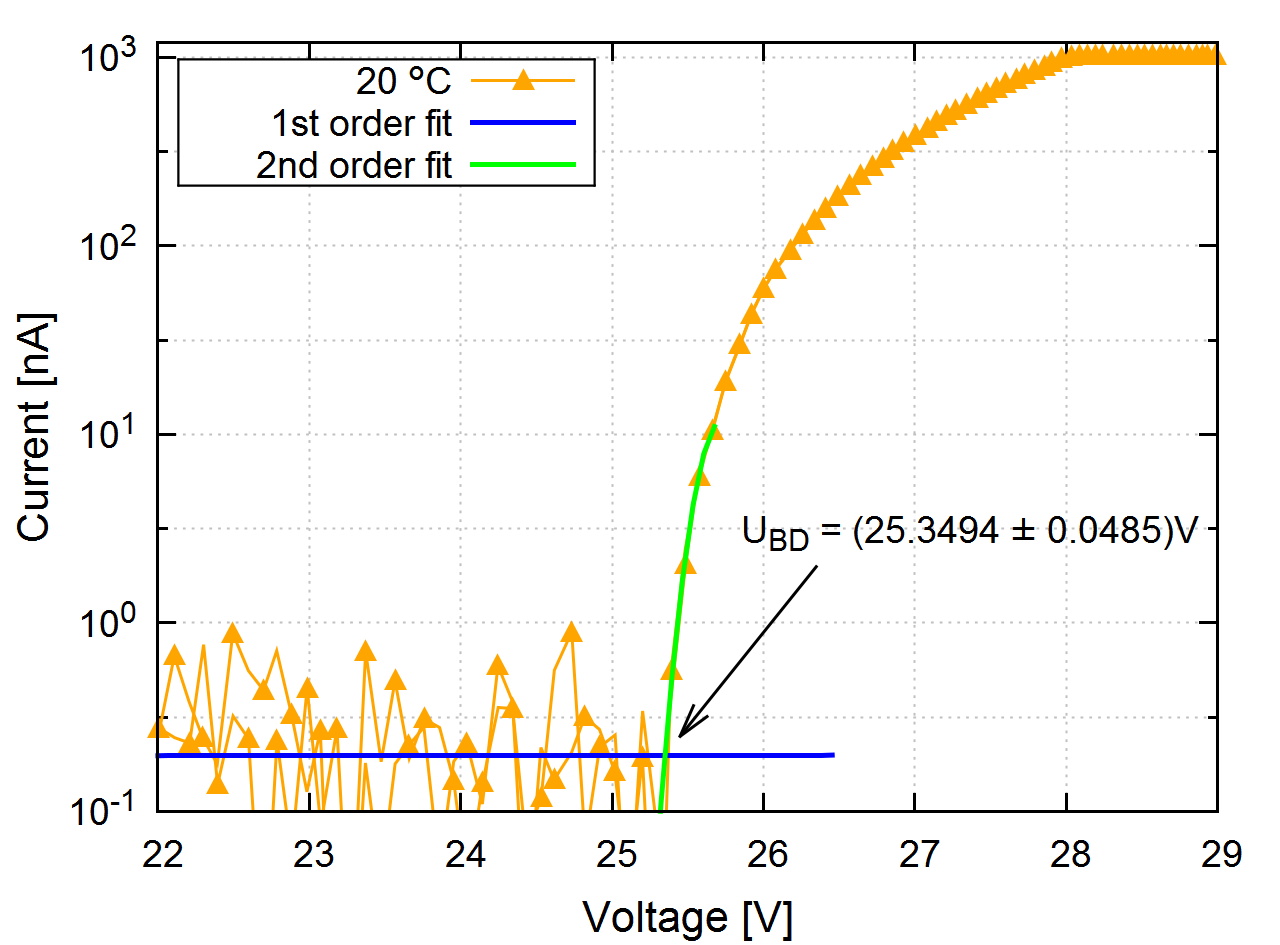
\includegraphics[width=0.49\textwidth]{./plots/iu_curve/1x1n2_bd_20.png}}
	\hfill
	\subfloat[(s)-configuration $\SI{15}{\degreeCelsius}$] {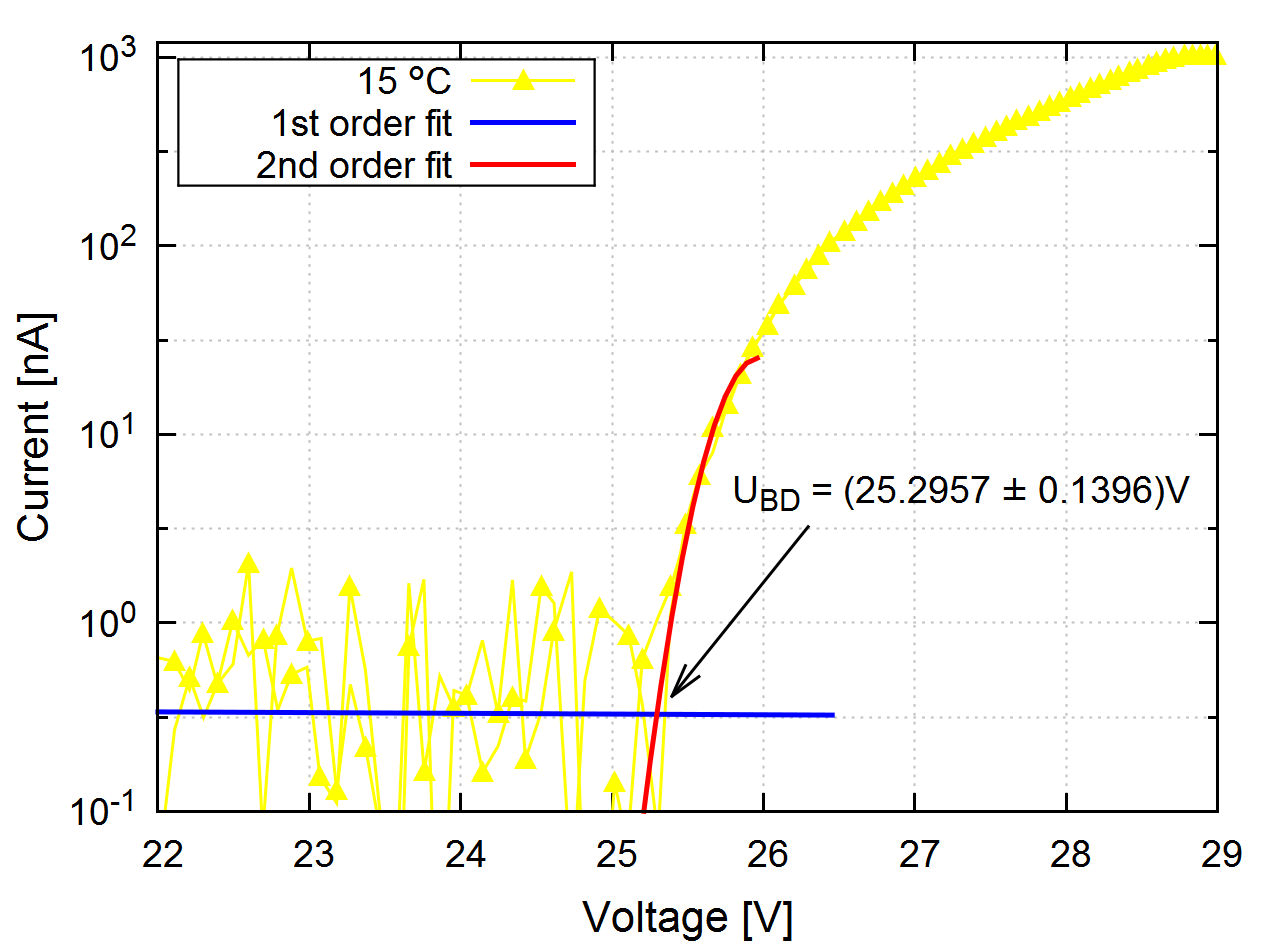
\includegraphics[width=0.49\textwidth]{./plots/iu_curve/1x1n2_bd_15.png}}
	\hfill
	\subfloat[(s)-configuration $\SI{10}{\degreeCelsius}$] {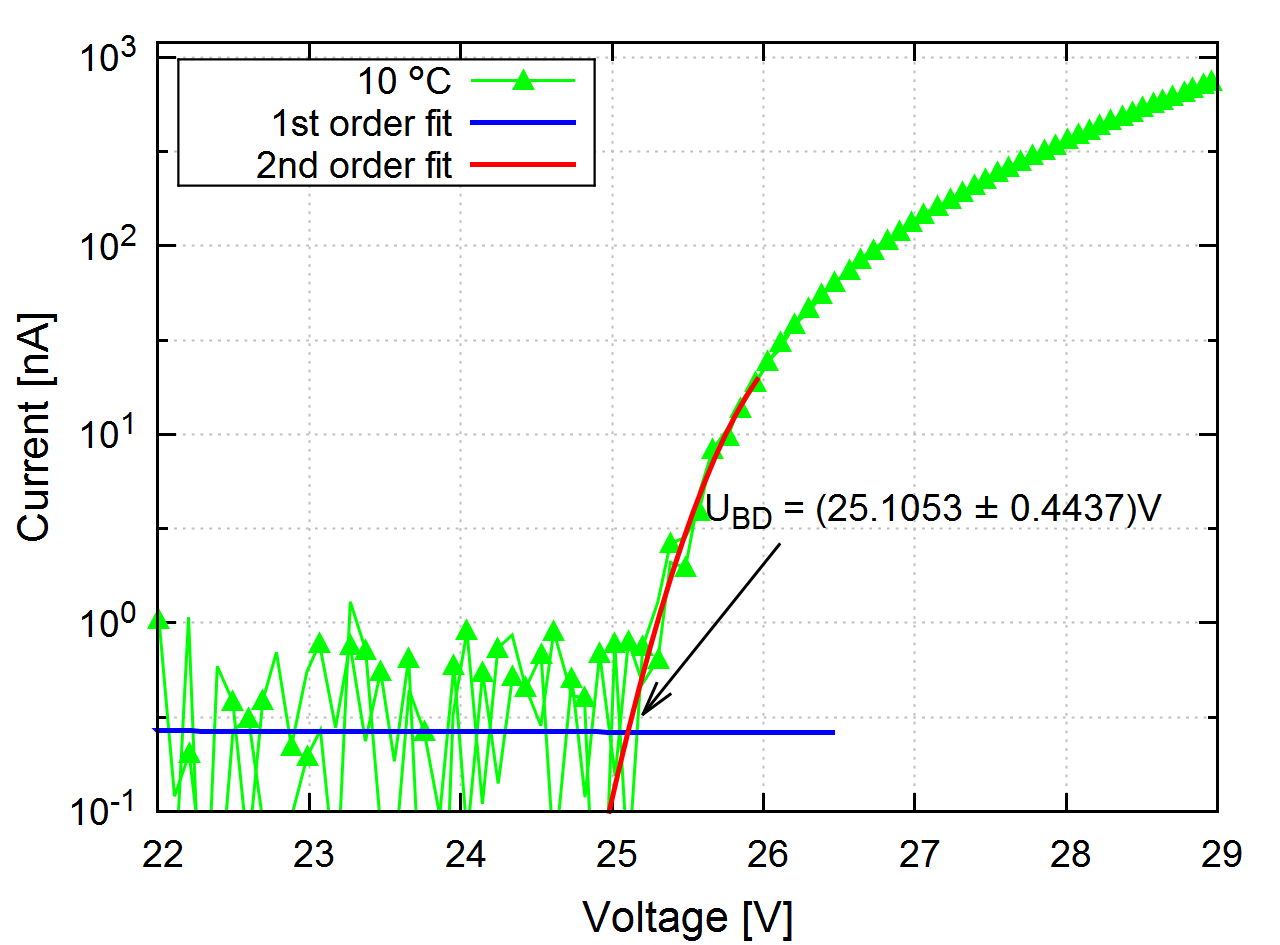
\includegraphics[width=0.49\textwidth]{./plots/iu_curve/1x1n2_bd_10.png}}
	\hfill
	\subfloat[(s)-configuration $\SI{5}{\degreeCelsius}$] {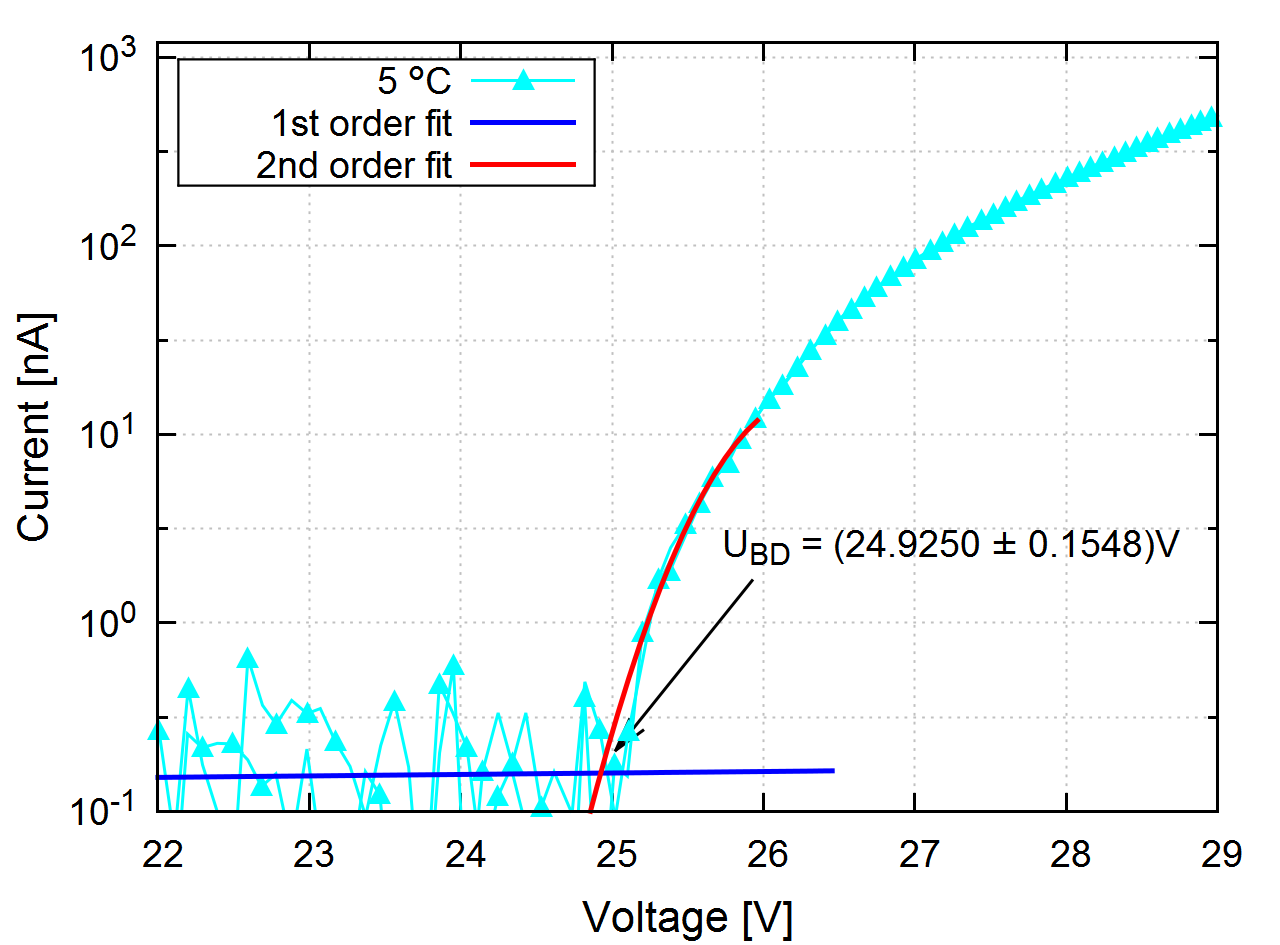
\includegraphics[width=0.49\textwidth]{./plots/iu_curve/1x1n2_bd_5.png}}
	\hfill
	\subfloat[(s)-configuration $\SI{0}{\degreeCelsius}$] {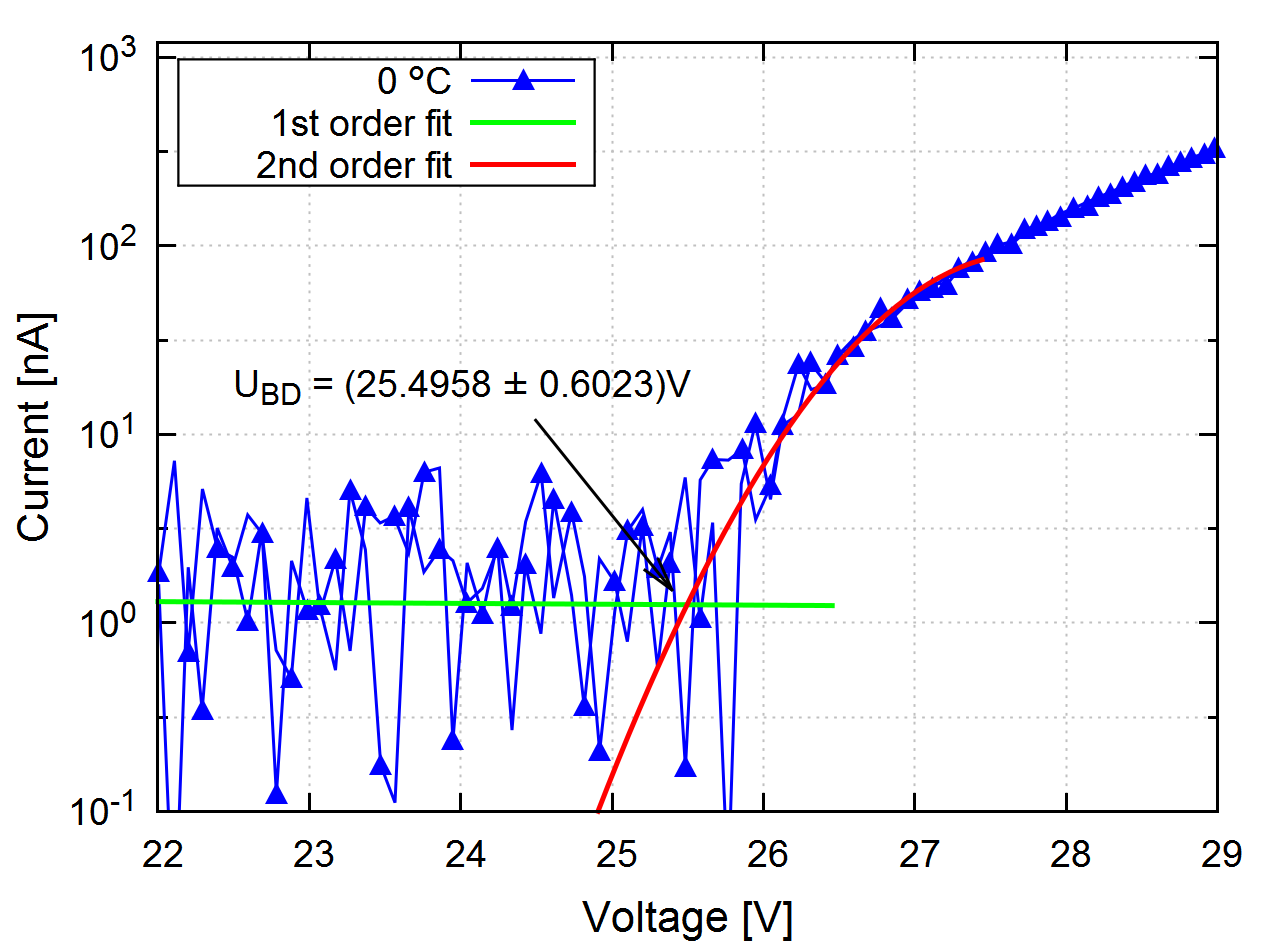
\includegraphics[width=0.49\textwidth]{./plots/iu_curve/1x1n2_bd_0.png}}
	\hfill
	\subfloat[(s)-configuration $\SI{-25}{\degreeCelsius}$] {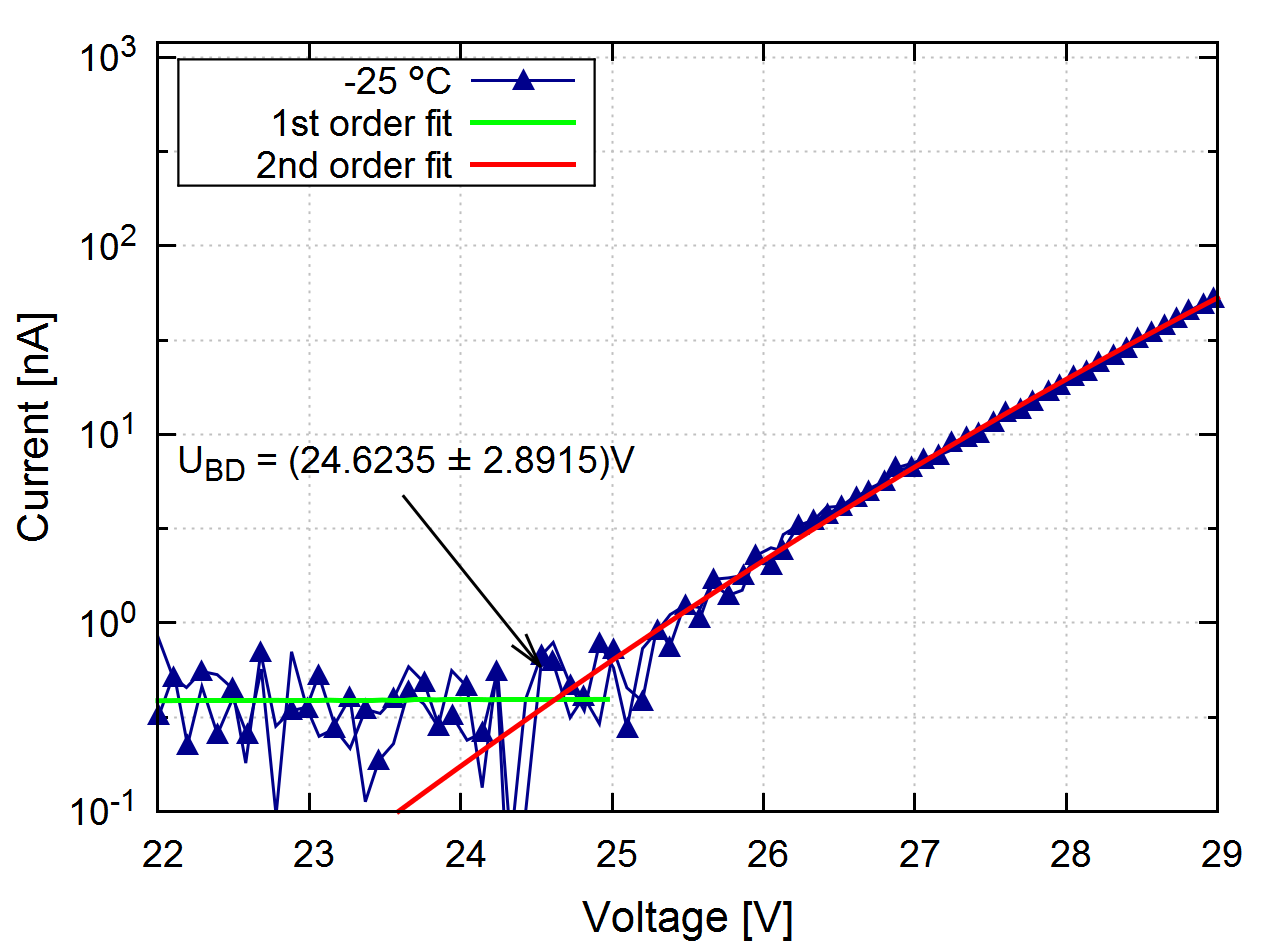
\includegraphics[width=0.38\textwidth]{./plots/iu_curve/1x1n2_bd_-25.png}}
	\hfill
	\caption[Breakdown fits (single)]{Fits for determining the breakdown of a single SiPM. }
	\label{ap:B:breakdown_fits_single}
\end{figure}

\newpage

\begin{figure}[H]
	\subfloat[(h)-configuration $\SI{25}{\degreeCelsius}$] {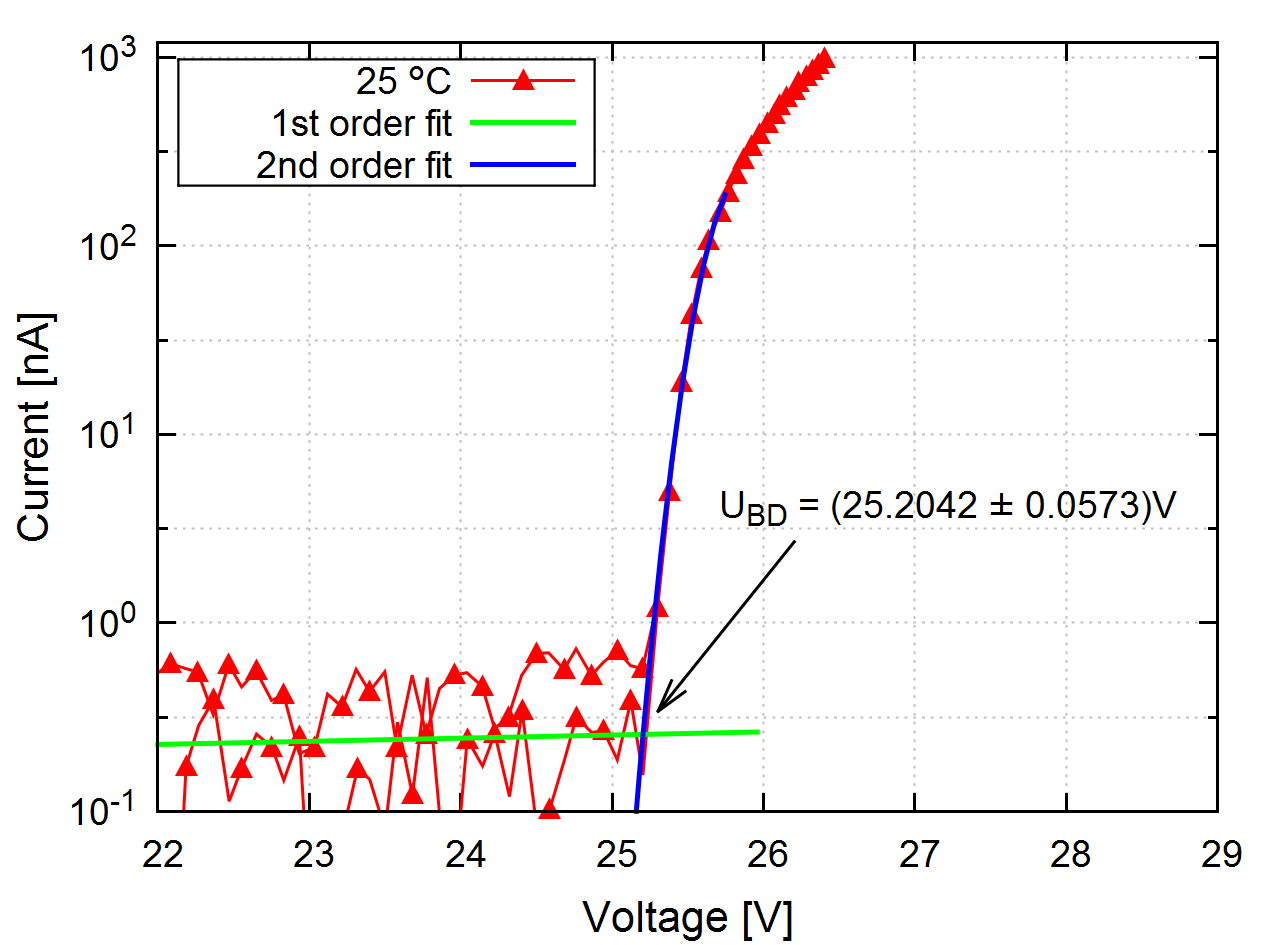
\includegraphics[width=0.49\textwidth]{./plots/iu_curve/4x1n6_bd_25.png}}
	\hfill
	\subfloat[(h)-configuration $\SI{20}{\degreeCelsius}$] {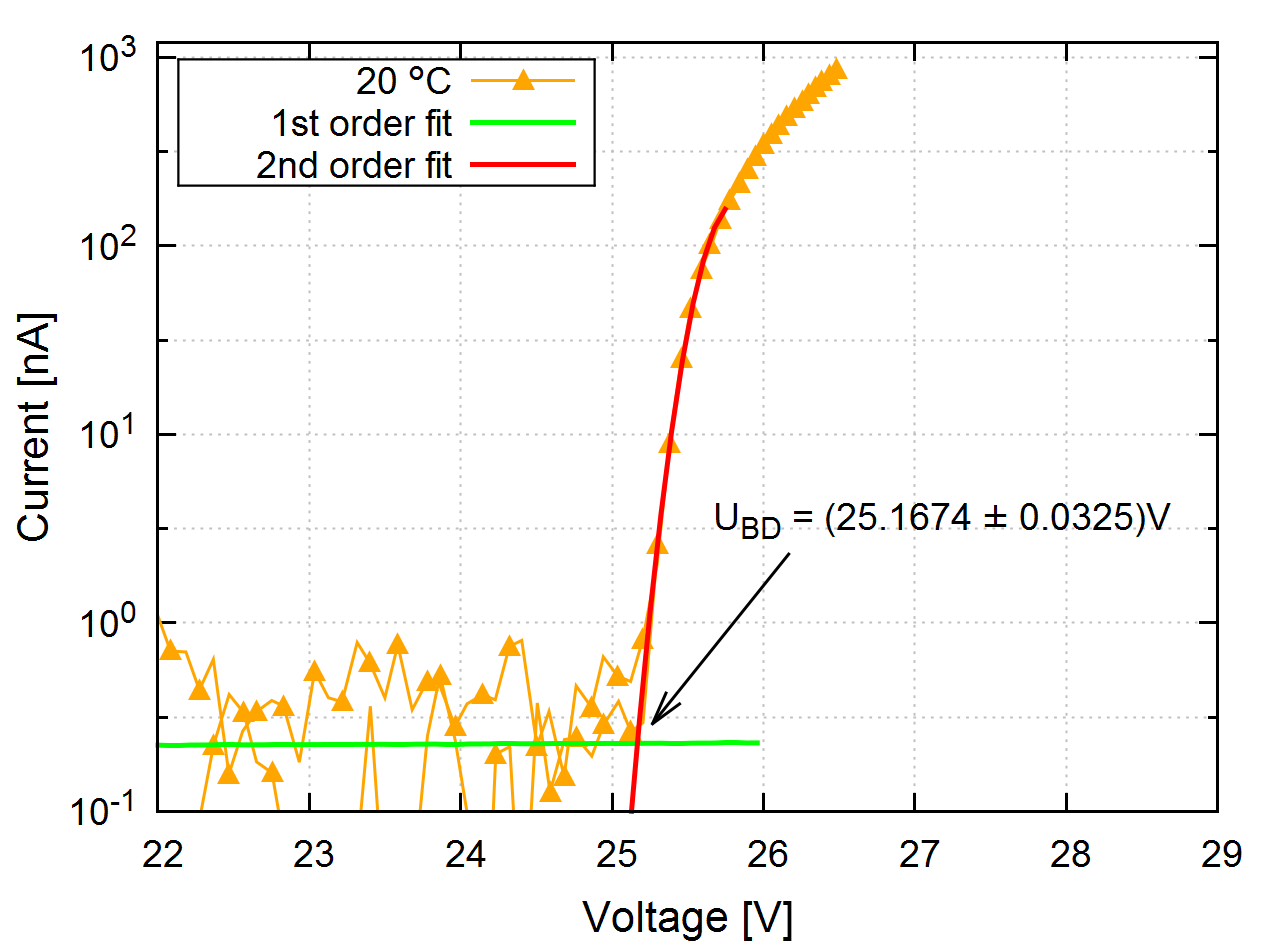
\includegraphics[width=0.49\textwidth]{./plots/iu_curve/4x1n6_bd_20.png}}
	\hfill
	\subfloat[(h)-configuration $\SI{15}{\degreeCelsius}$] {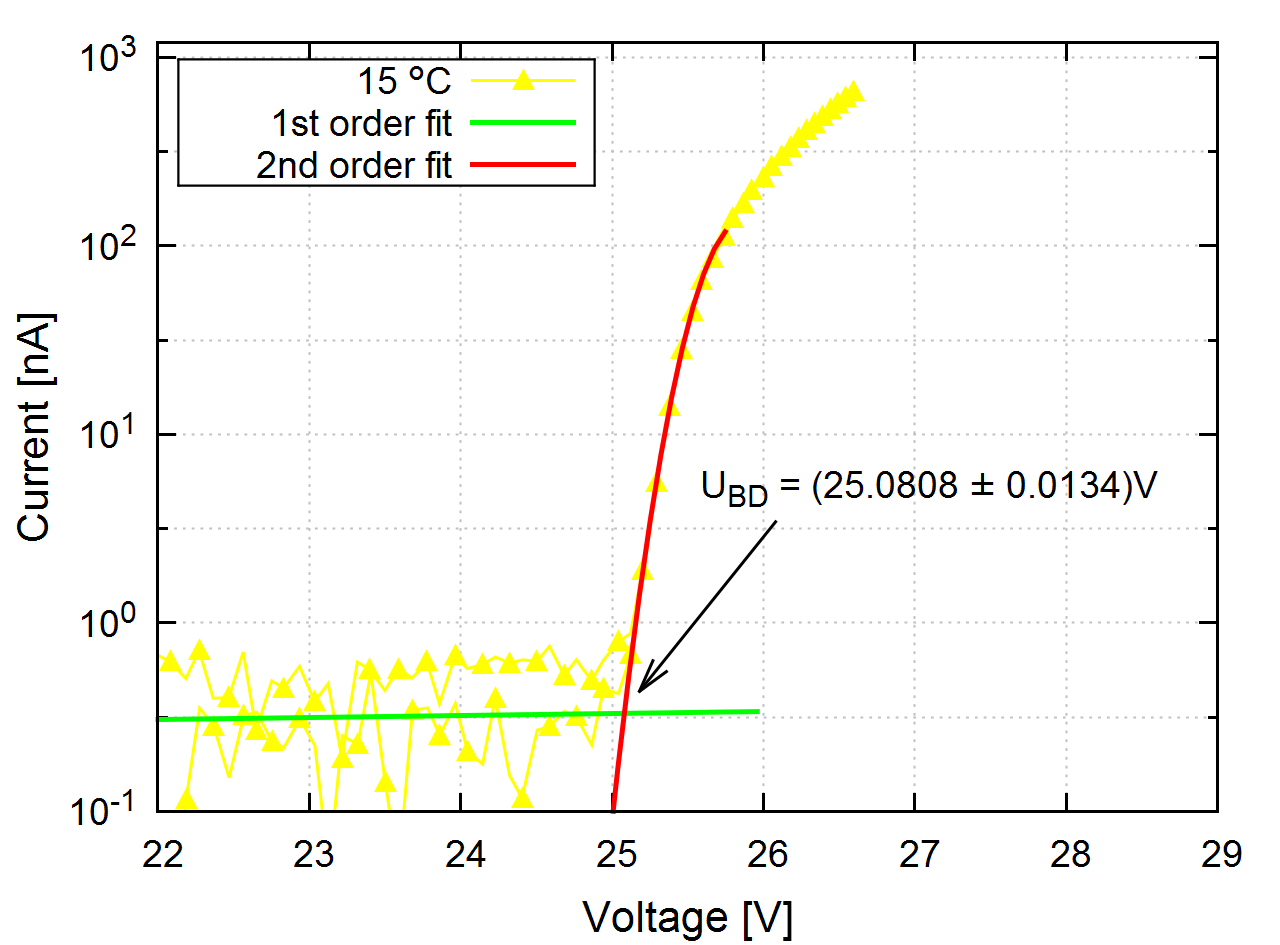
\includegraphics[width=0.49\textwidth]{./plots/iu_curve/4x1n6_bd_15.png}}
	\hfill
	\subfloat[(h)-configuration $\SI{10}{\degreeCelsius}$] {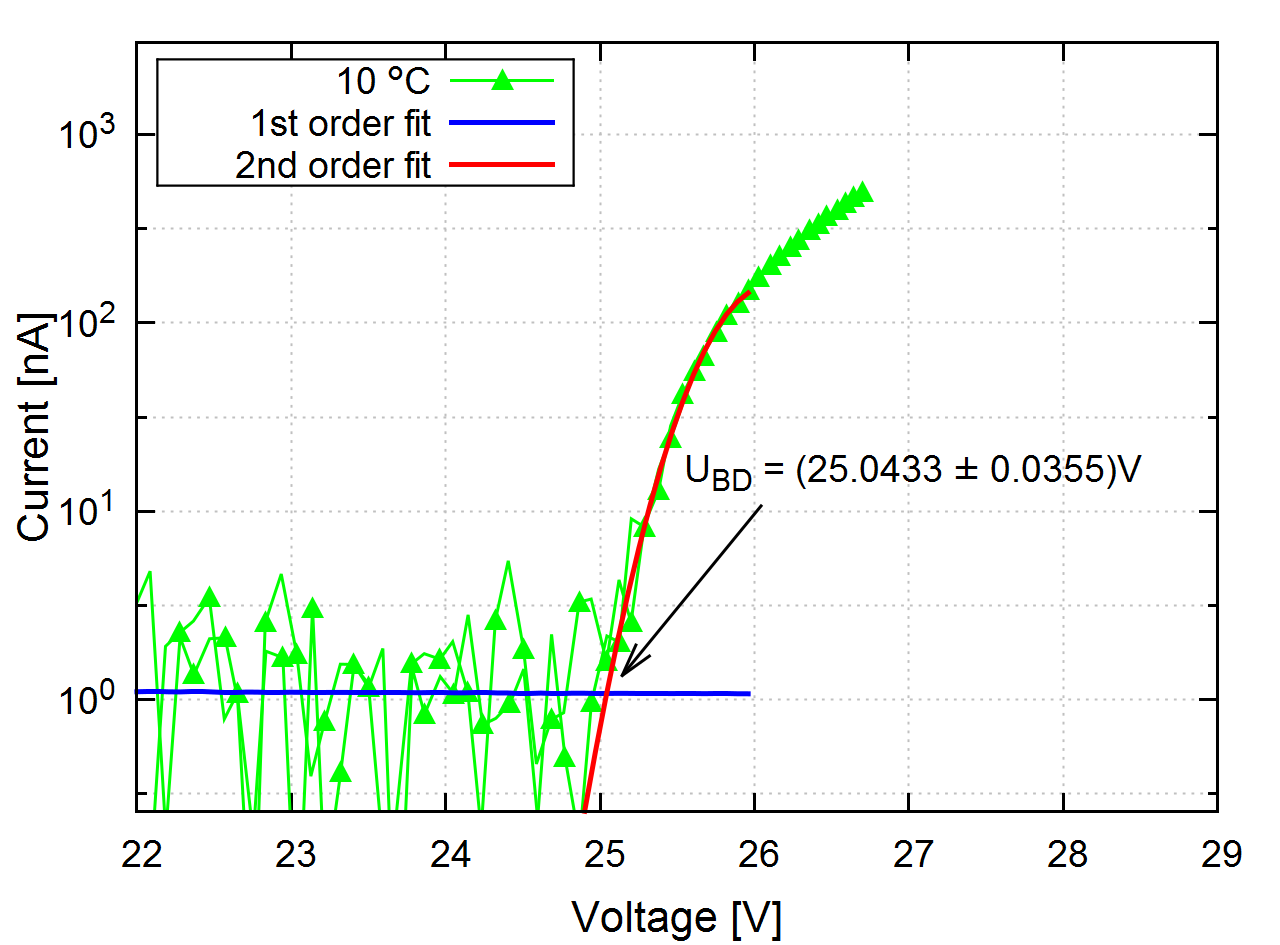
\includegraphics[width=0.49\textwidth]{./plots/iu_curve/4x1n6_bd_10.png}}
	\hfill
	\subfloat[(h)-configuration $\SI{5}{\degreeCelsius}$] {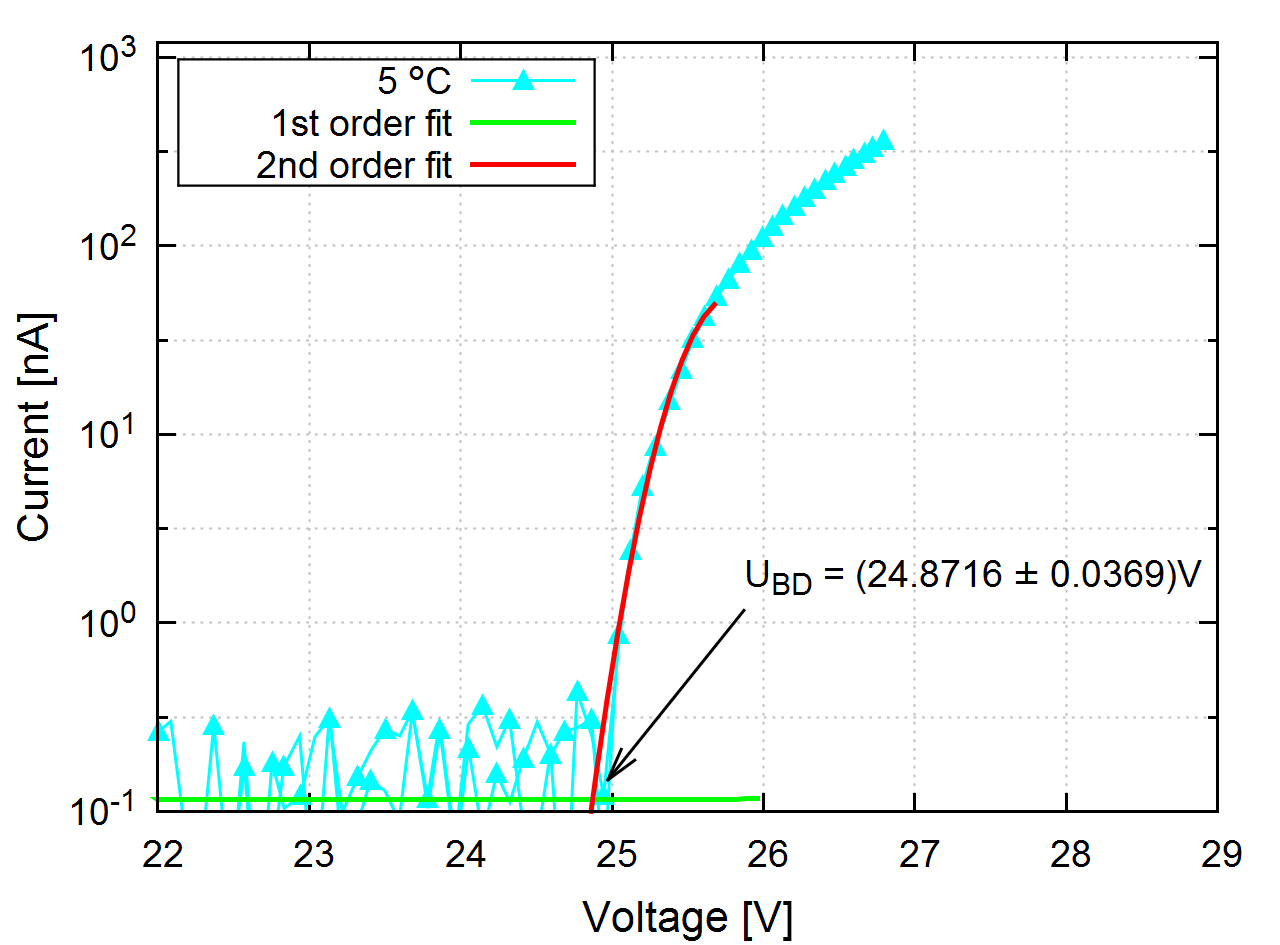
\includegraphics[width=0.49\textwidth]{./plots/iu_curve/4x1n6_bd_5.png}}
	\hfill
	\subfloat[(h)-configuration $\SI{0}{\degreeCelsius}$] {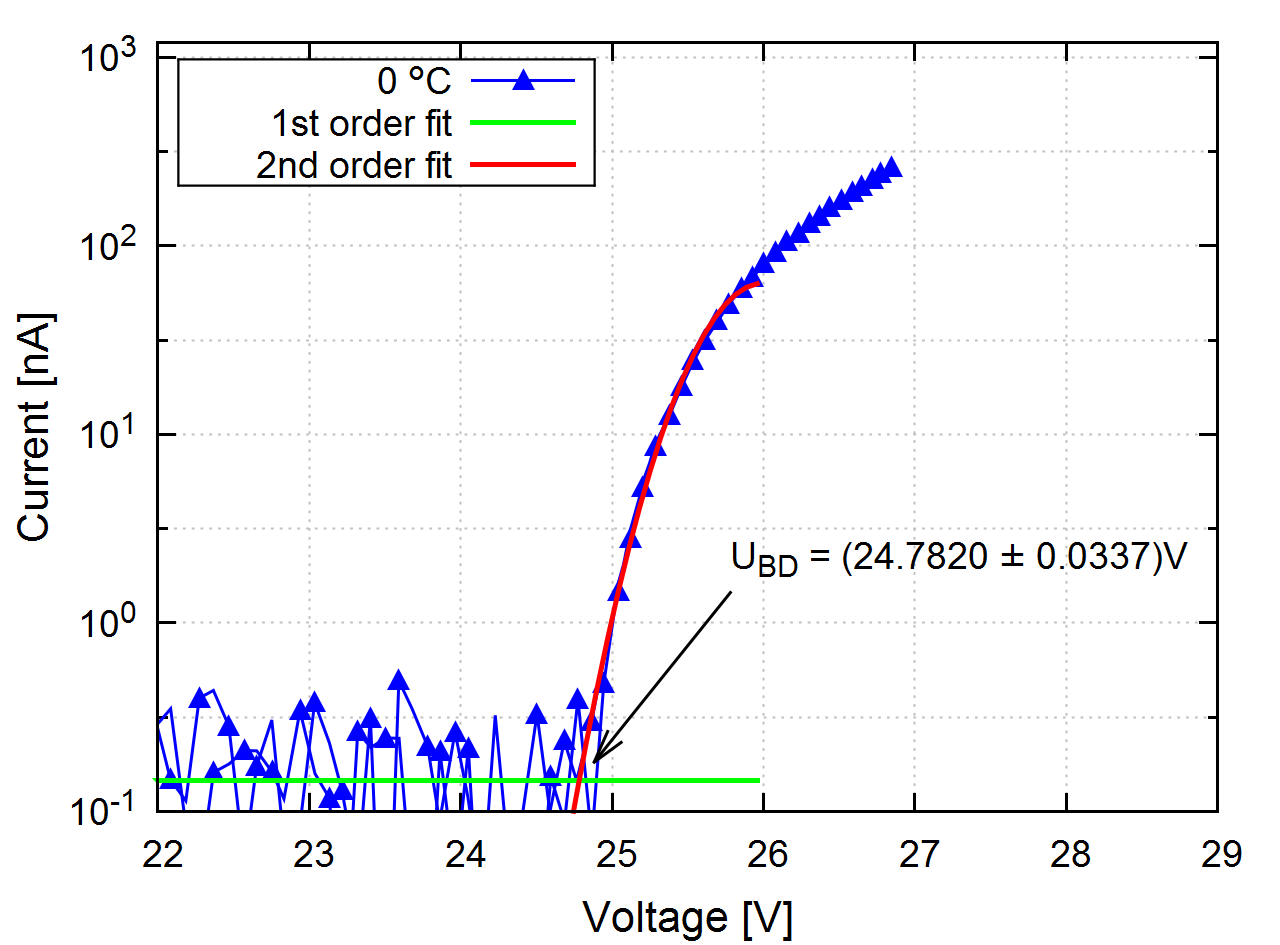
\includegraphics[width=0.49\textwidth]{./plots/iu_curve/4x1n6_bd_0.png}}
	\hfill
	\subfloat[(h)-configuration $\SI{-25}{\degreeCelsius}$] {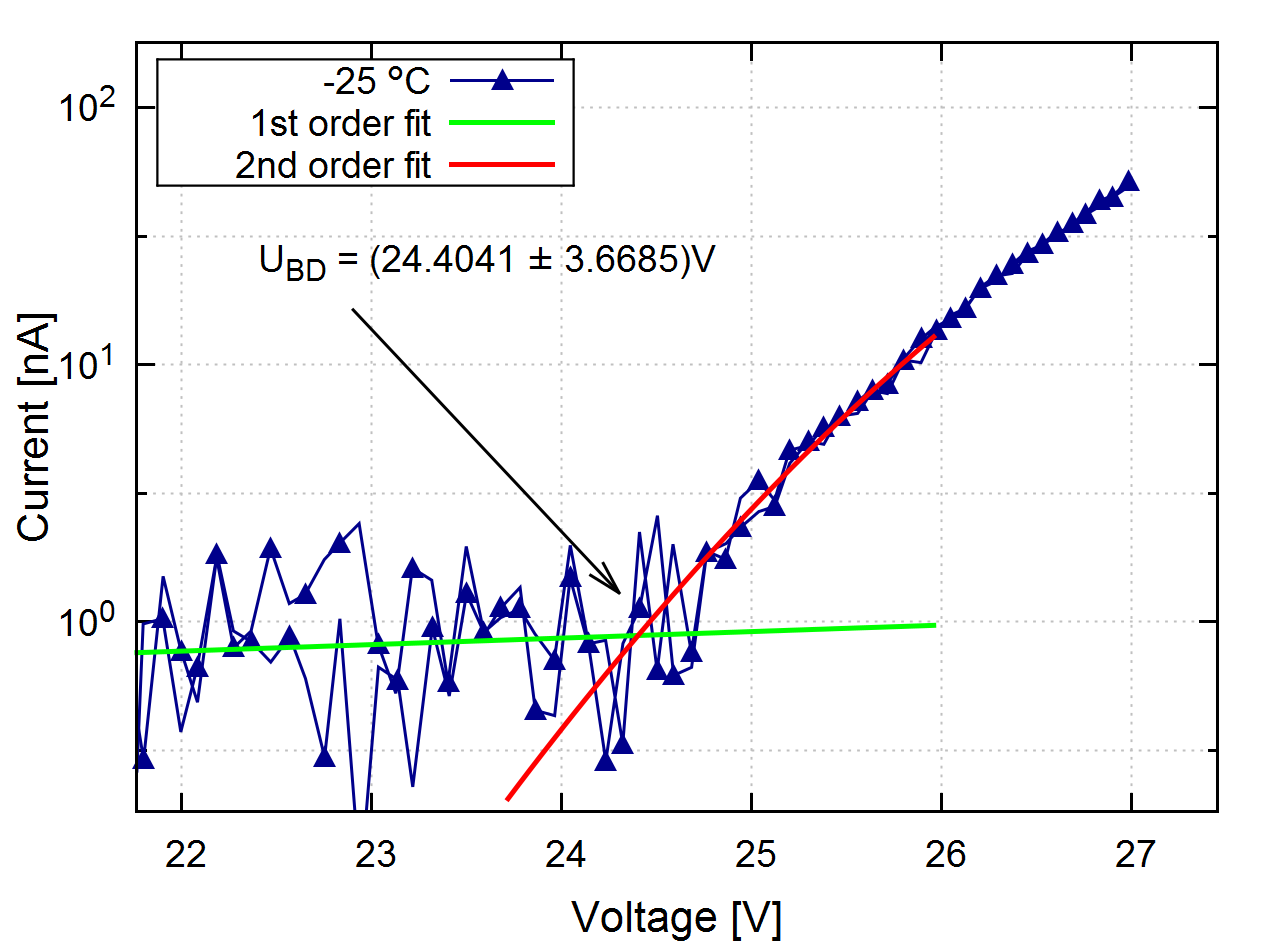
\includegraphics[width=0.38\textwidth]{./plots/iu_curve/4x1n6_bd_-25.png}}
	\hfill
	\caption[Breakdown fits (hybrid)]{Fits for determining the breakdown of a hybrid board. }
	\label{ap:B:breakdown_fits_hybrid}
\end{figure}

\newpage

\section{Operation voltage}

The relative slope $\dv{I}{V}\frac{1}{I(V)}$ shows a minimum some volts beyond breakdown. A second order polynomial function was used for determining the minimum:
\begin{align*}
I(V)&=A\cdot V^2+B\cdot V+C.
\end{align*}
The minimum can be found by deriving and zeroing:
\begin{align*}
\dv{I(V)}{V}&\overset{!}{=}0 \\
\Rightarrow V_0&=-\frac{B}{2A}.
\end{align*}
The error is again calculated by error propagation 
\begin{align*}
\Delta V_0=\arrowvert\dv{V_0}{A}\arrowvert\Delta A+\arrowvert\dv{V_0}{B}\arrowvert\Delta B.
\end{align*}
The fits can be found in figures \ref{ap:B:optimal_fits_single} and \ref{ap:B:optimal_fits_hybrid}.

\newpage

\begin{figure}[H]
	\subfloat[(s)-configuration $\SI{25}{\degreeCelsius}$] {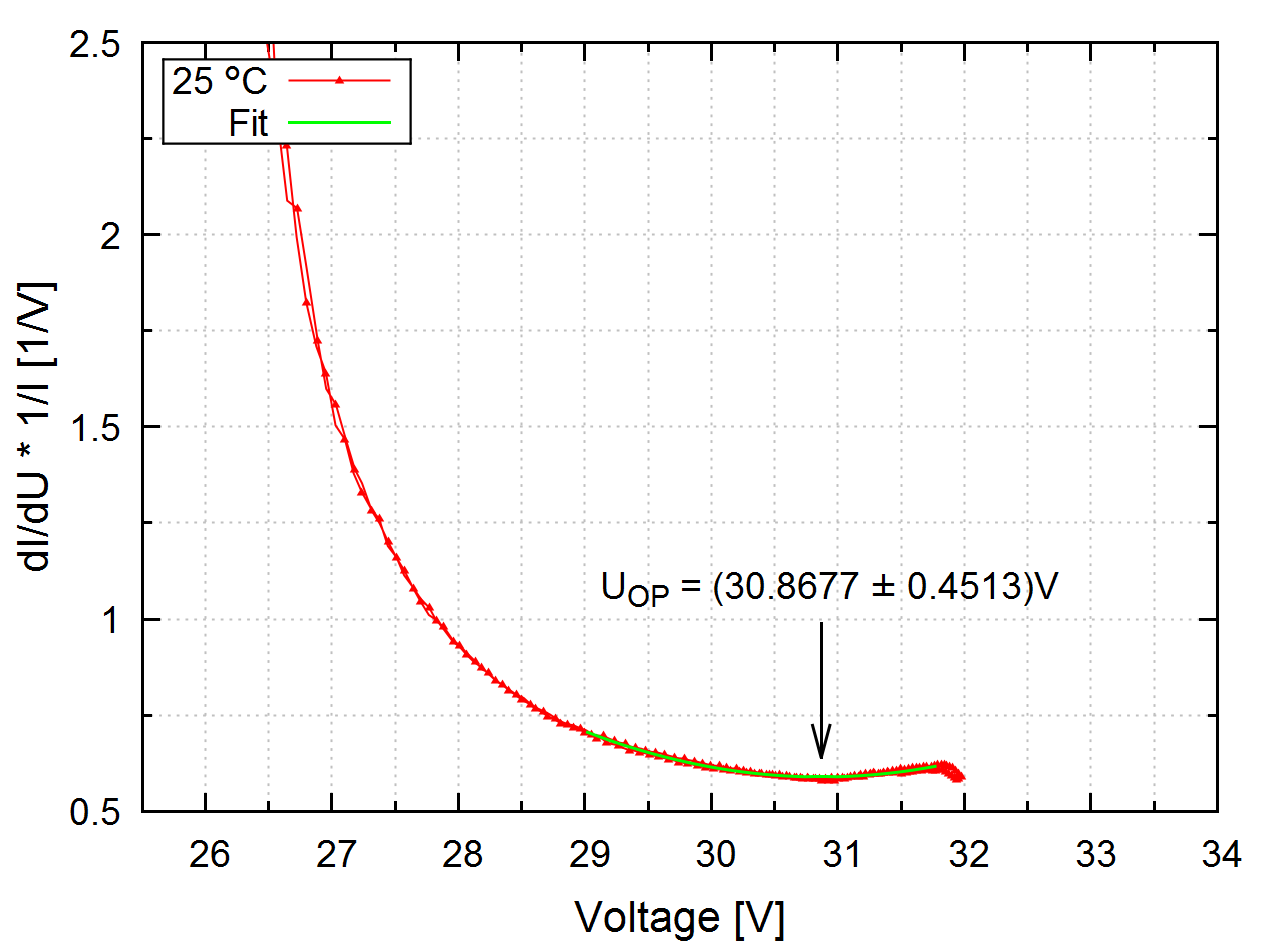
\includegraphics[width=0.49\textwidth]{./plots/iu_curve/1x1n2_op_25.png}}
	\hfill
	\subfloat[(s)-configuration $\SI{20}{\degreeCelsius}$] {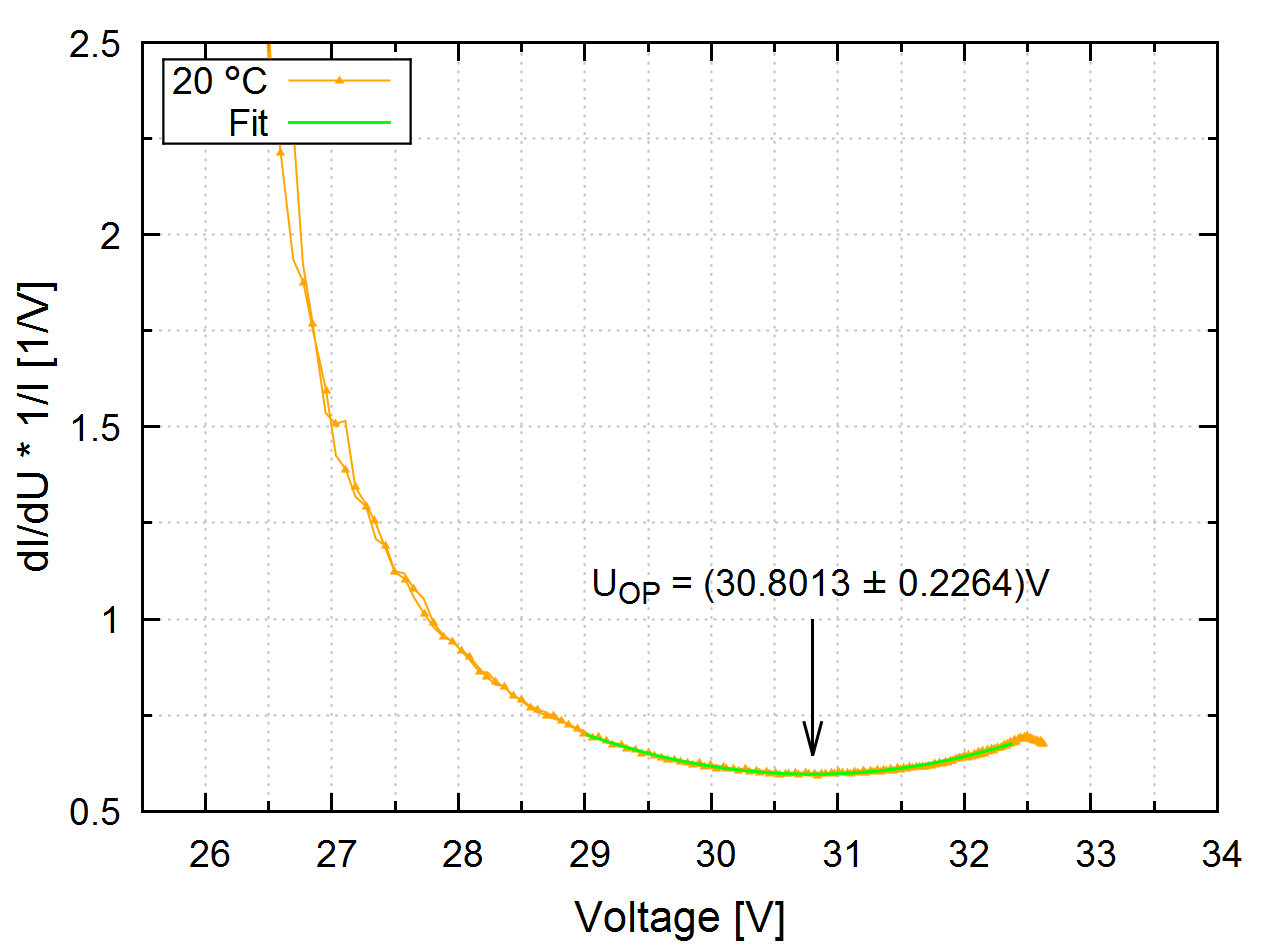
\includegraphics[width=0.49\textwidth]{./plots/iu_curve/1x1n2_op_20.png}}
	\hfill
	\subfloat[(s)-configuration $\SI{15}{\degreeCelsius}$] {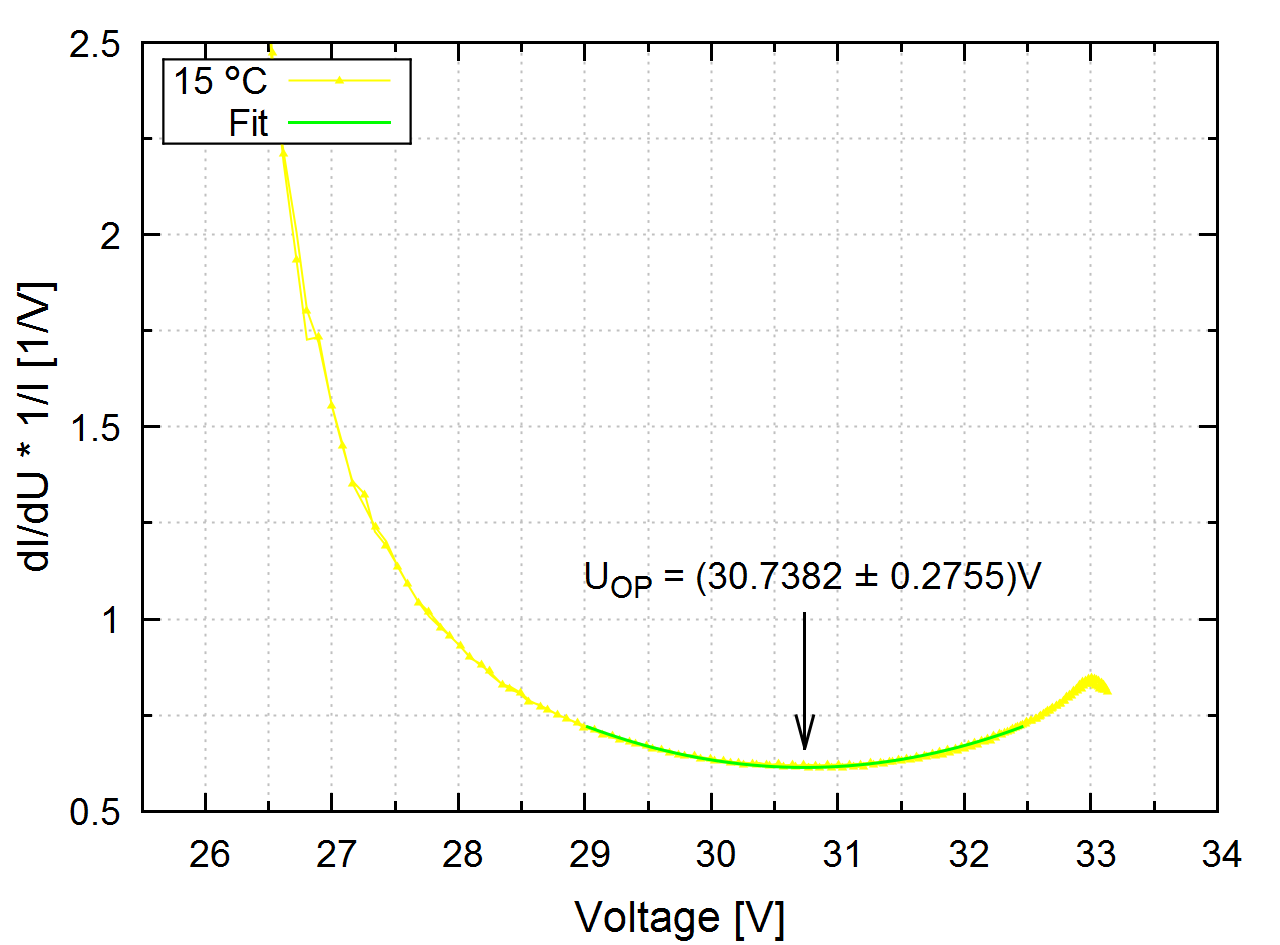
\includegraphics[width=0.49\textwidth]{./plots/iu_curve/1x1n2_op_15.png}}
	\hfill
	\subfloat[(s)-configuration $\SI{10}{\degreeCelsius}$] {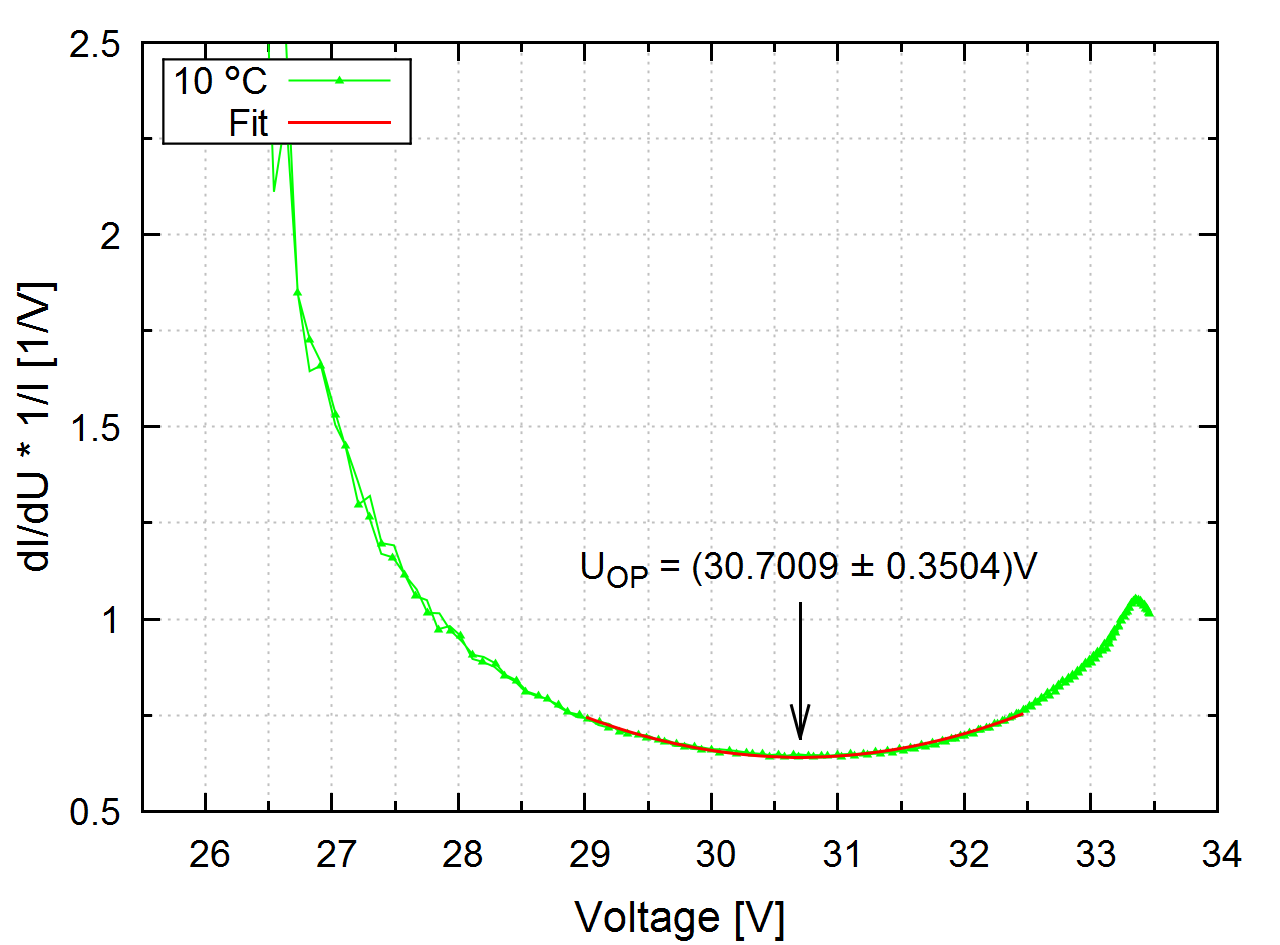
\includegraphics[width=0.49\textwidth]{./plots/iu_curve/1x1n2_op_10.png}}
	\hfill
	\subfloat[(s)-configuration $\SI{5}{\degreeCelsius}$] {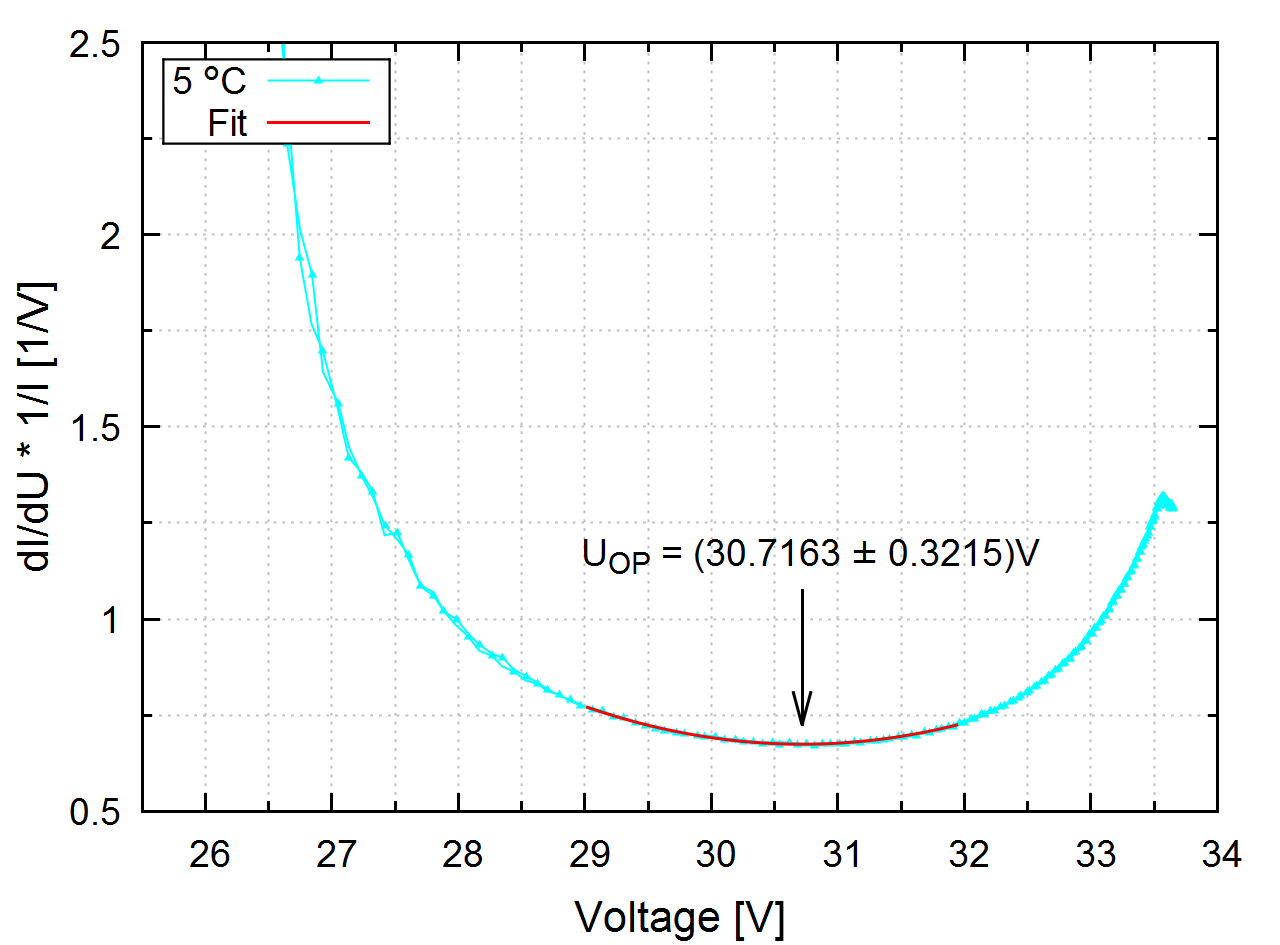
\includegraphics[width=0.49\textwidth]{./plots/iu_curve/1x1n2_op_5.png}}
	\hfill
	\subfloat[(s)-configuration $\SI{0}{\degreeCelsius}$] {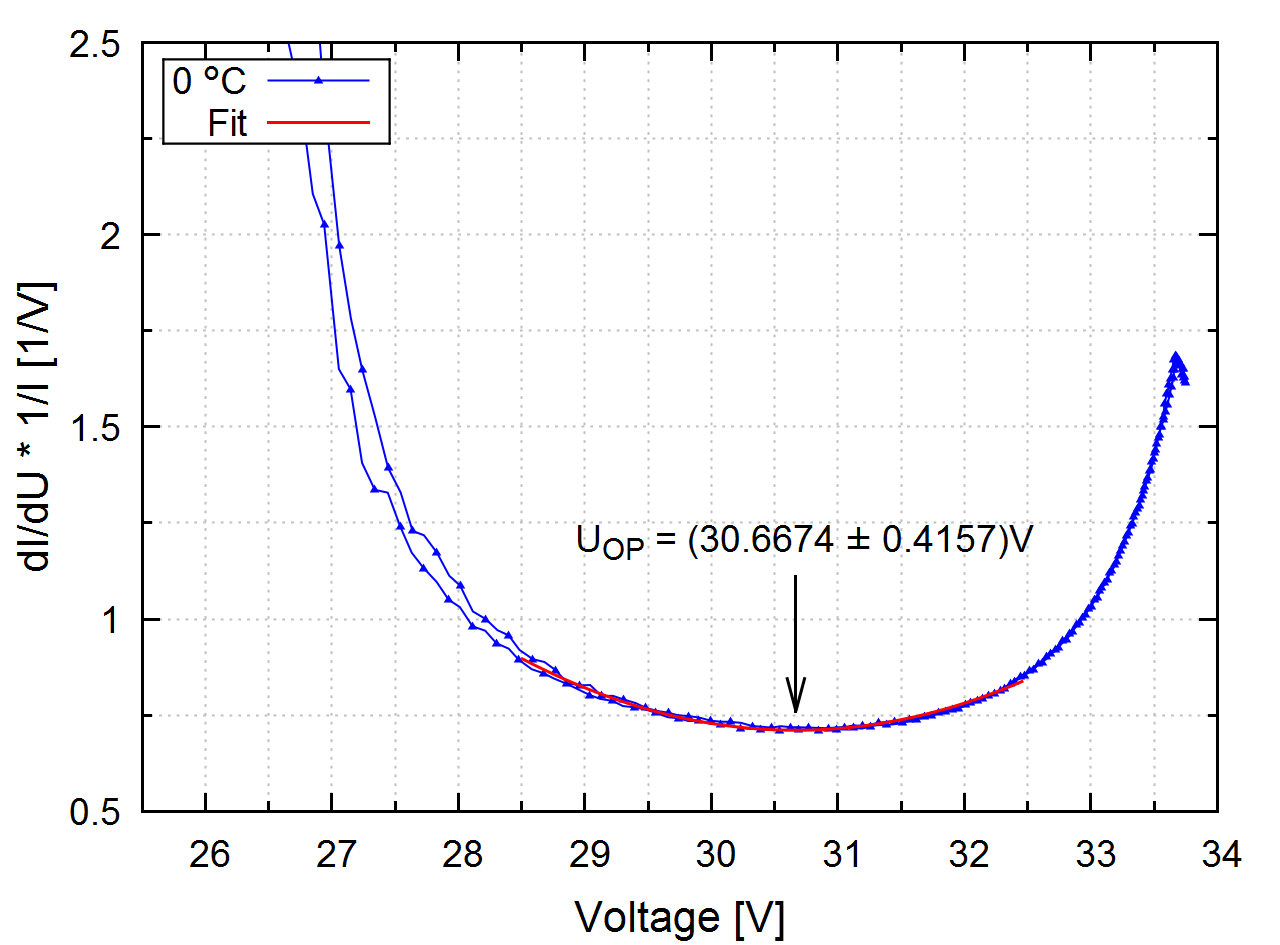
\includegraphics[width=0.49\textwidth]{./plots/iu_curve/1x1n2_op_0.png}}
	\hfill
	\subfloat[(s)-configuration $\SI{-25}{\degreeCelsius}$] {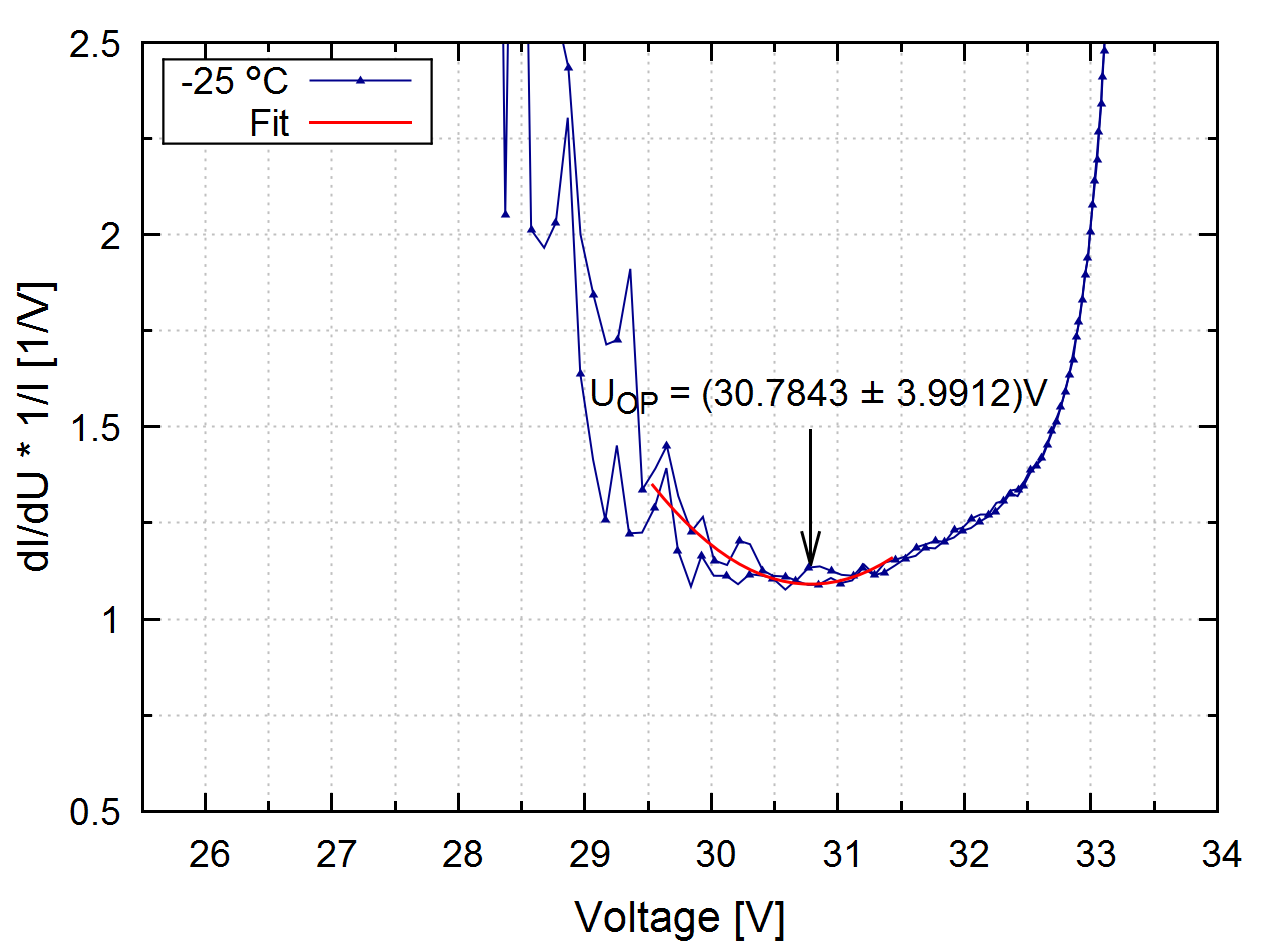
\includegraphics[width=0.38\textwidth]{./plots/iu_curve/1x1n2_op_-25.png}}
	\hfill
	\caption[Operation voltage fits (single)]{Fits for determining the operation voltage of a single SiPM. }
	\label{ap:B:optimal_fits_single}
\end{figure}

\newpage

\begin{figure}[H]
	\subfloat[(s)-configuration $\SI{25}{\degreeCelsius}$] {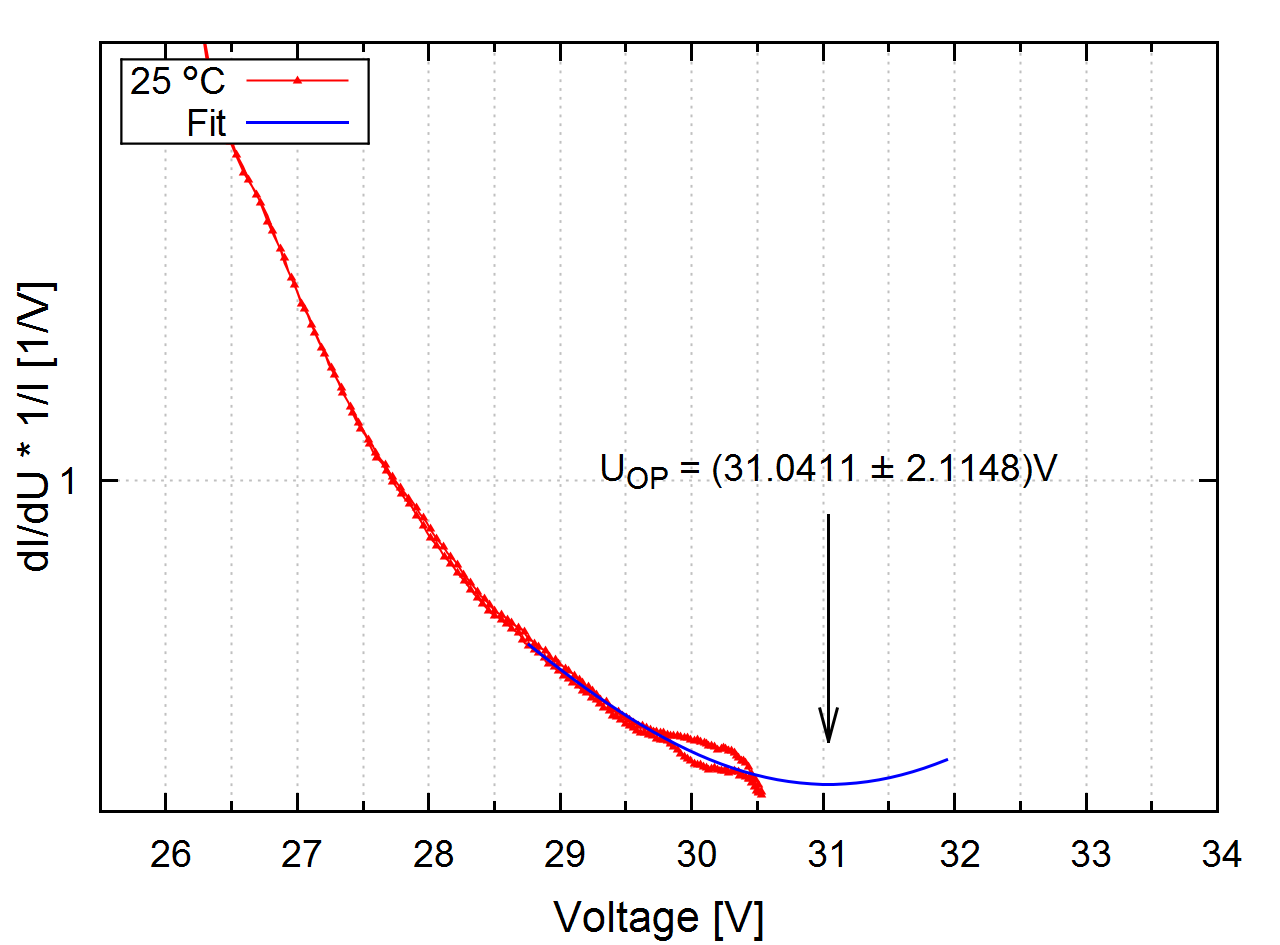
\includegraphics[width=0.49\textwidth]{./plots/iu_curve/4x1n6_op_25.png}}
	\hfill
	\subfloat[(s)-configuration $\SI{20}{\degreeCelsius}$] {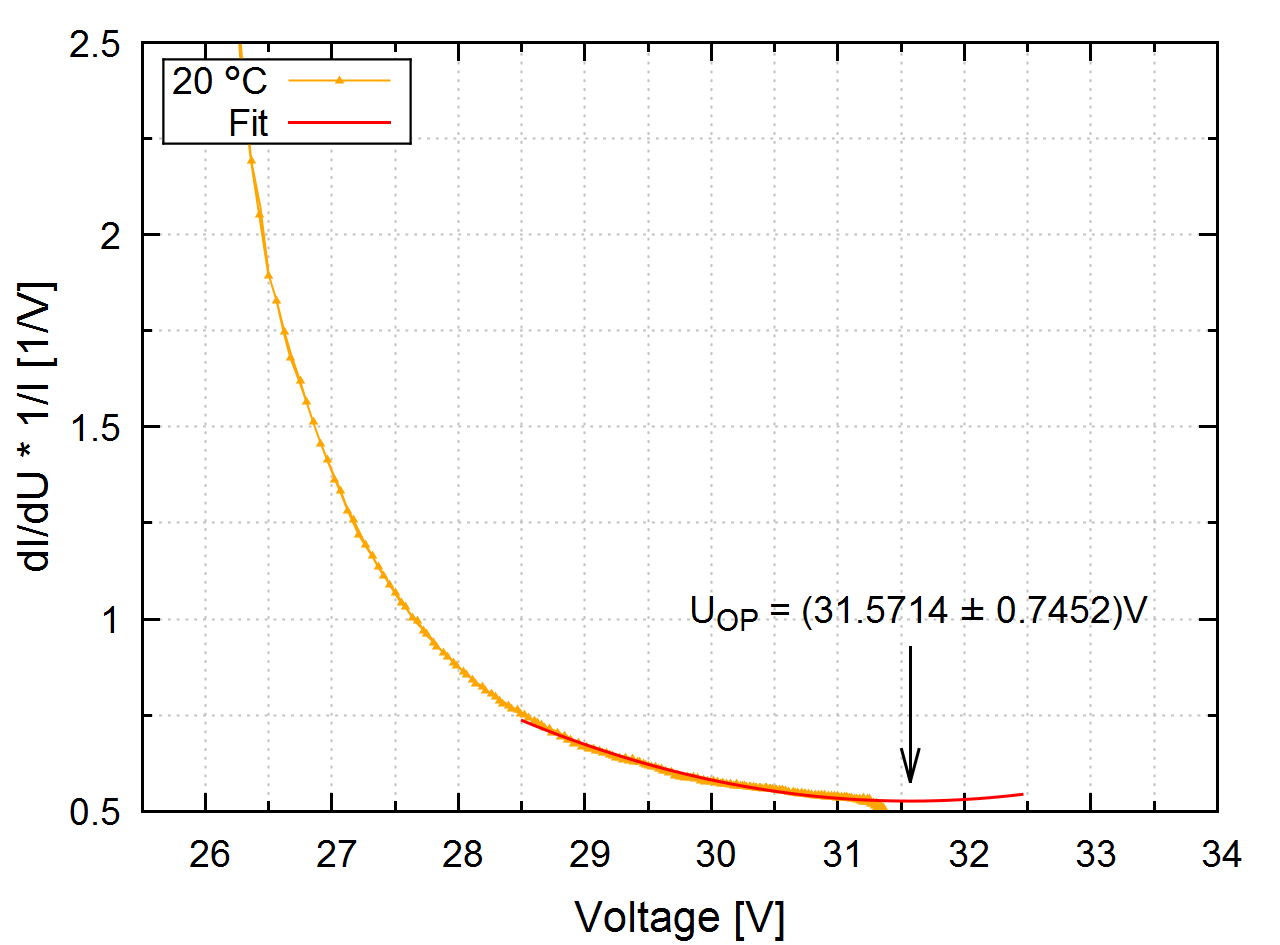
\includegraphics[width=0.49\textwidth]{./plots/iu_curve/4x1n6_op_20.png}}
	\hfill
	\subfloat[(s)-configuration $\SI{15}{\degreeCelsius}$] {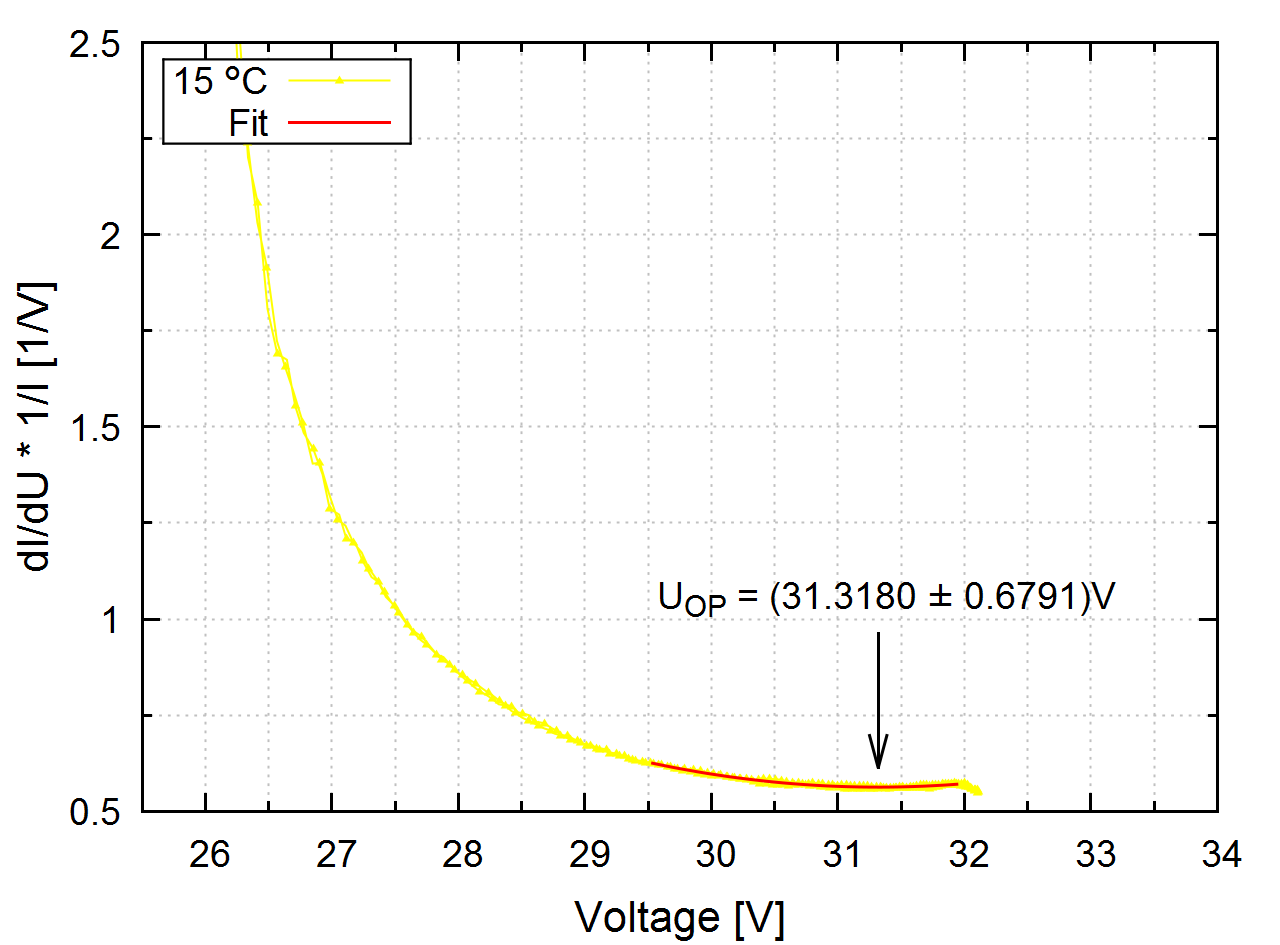
\includegraphics[width=0.49\textwidth]{./plots/iu_curve/4x1n6_op_15.png}}
	\hfill
	\subfloat[(s)-configuration $\SI{10}{\degreeCelsius}$] {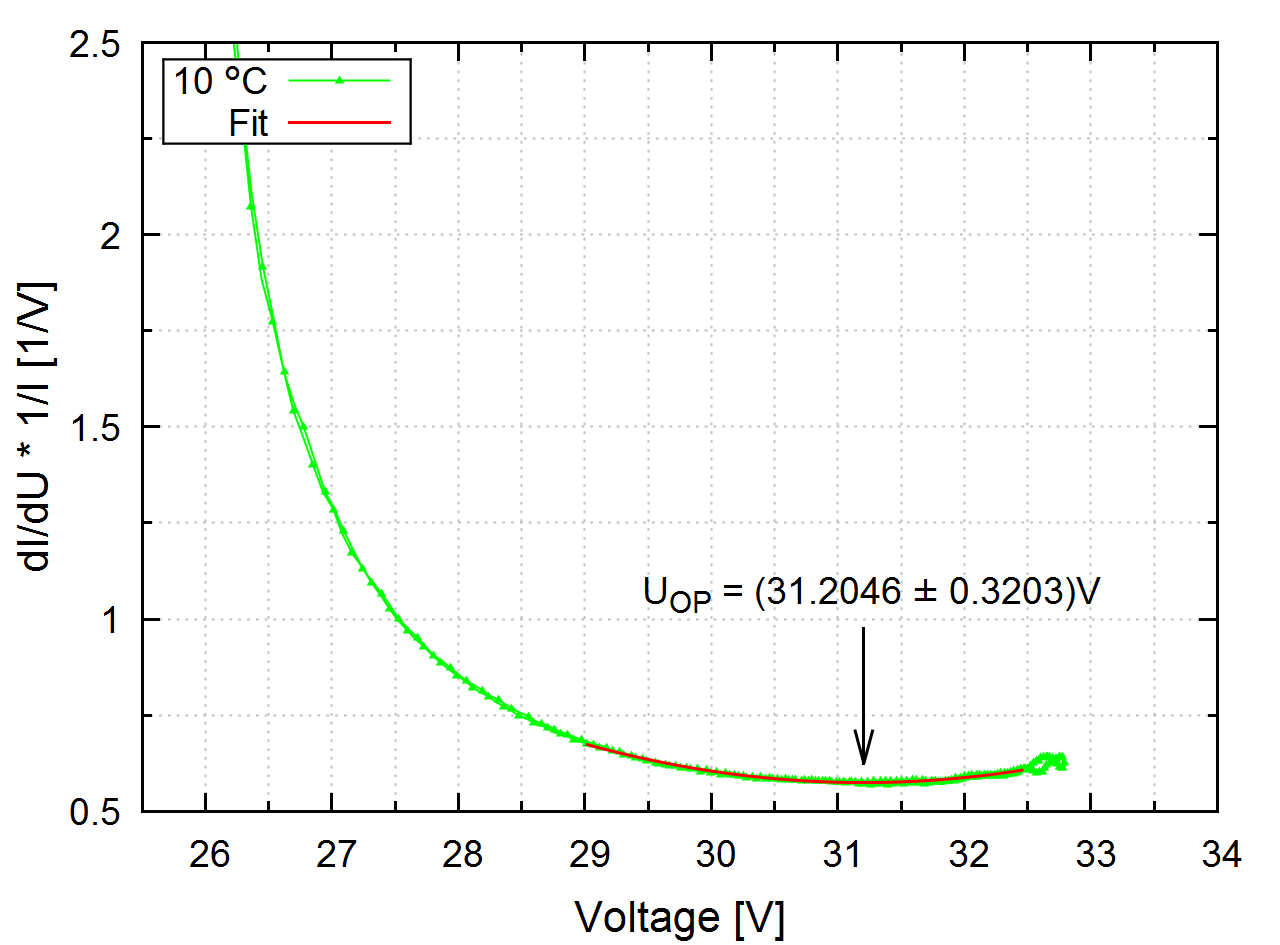
\includegraphics[width=0.49\textwidth]{./plots/iu_curve/4x1n6_op_10.png}}
	\hfill
	\subfloat[(s)-configuration $\SI{5}{\degreeCelsius}$] {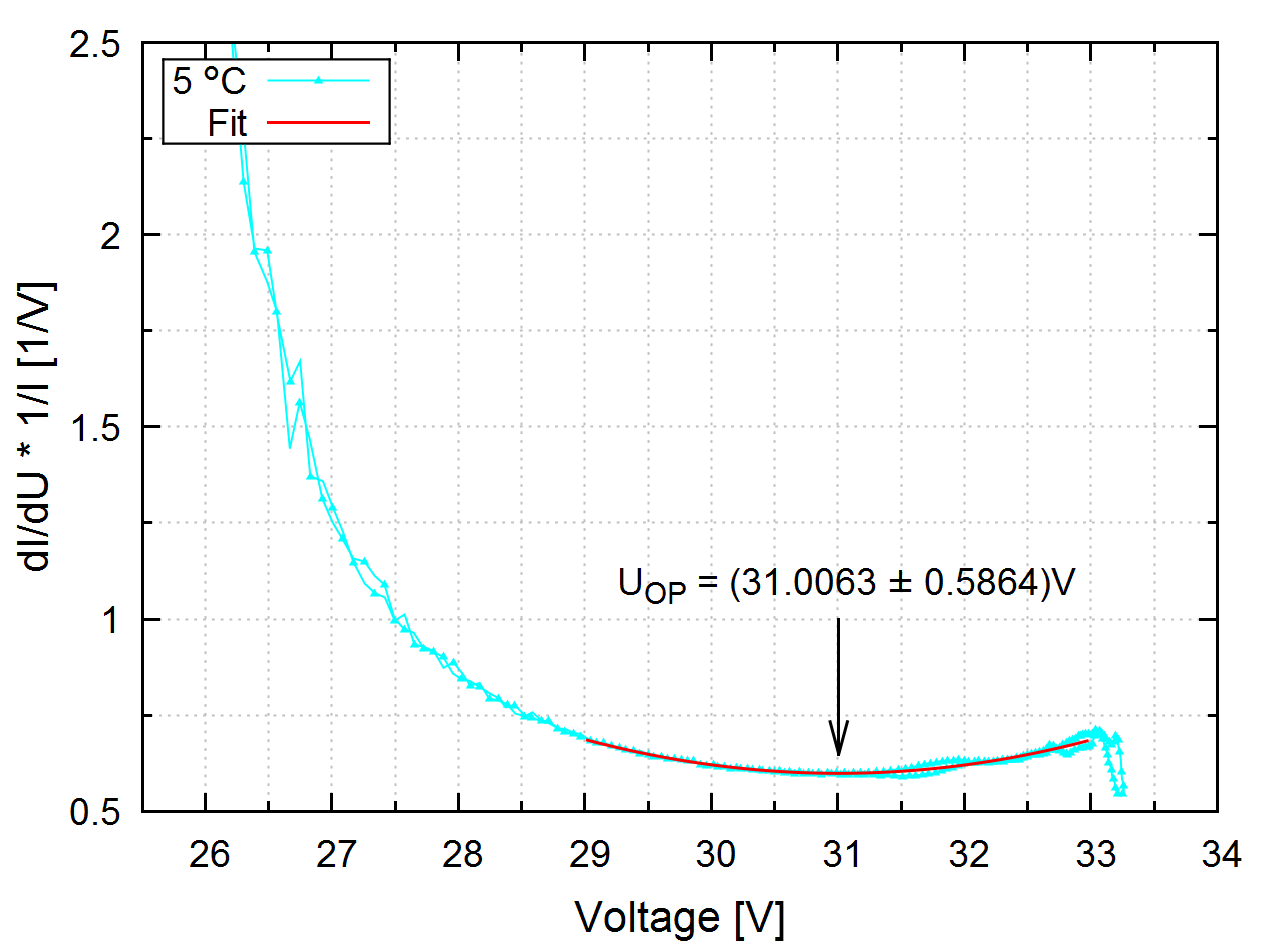
\includegraphics[width=0.49\textwidth]{./plots/iu_curve/4x1n6_op_5.png}}
	\hfill
	\subfloat[(s)-configuration $\SI{0}{\degreeCelsius}$] {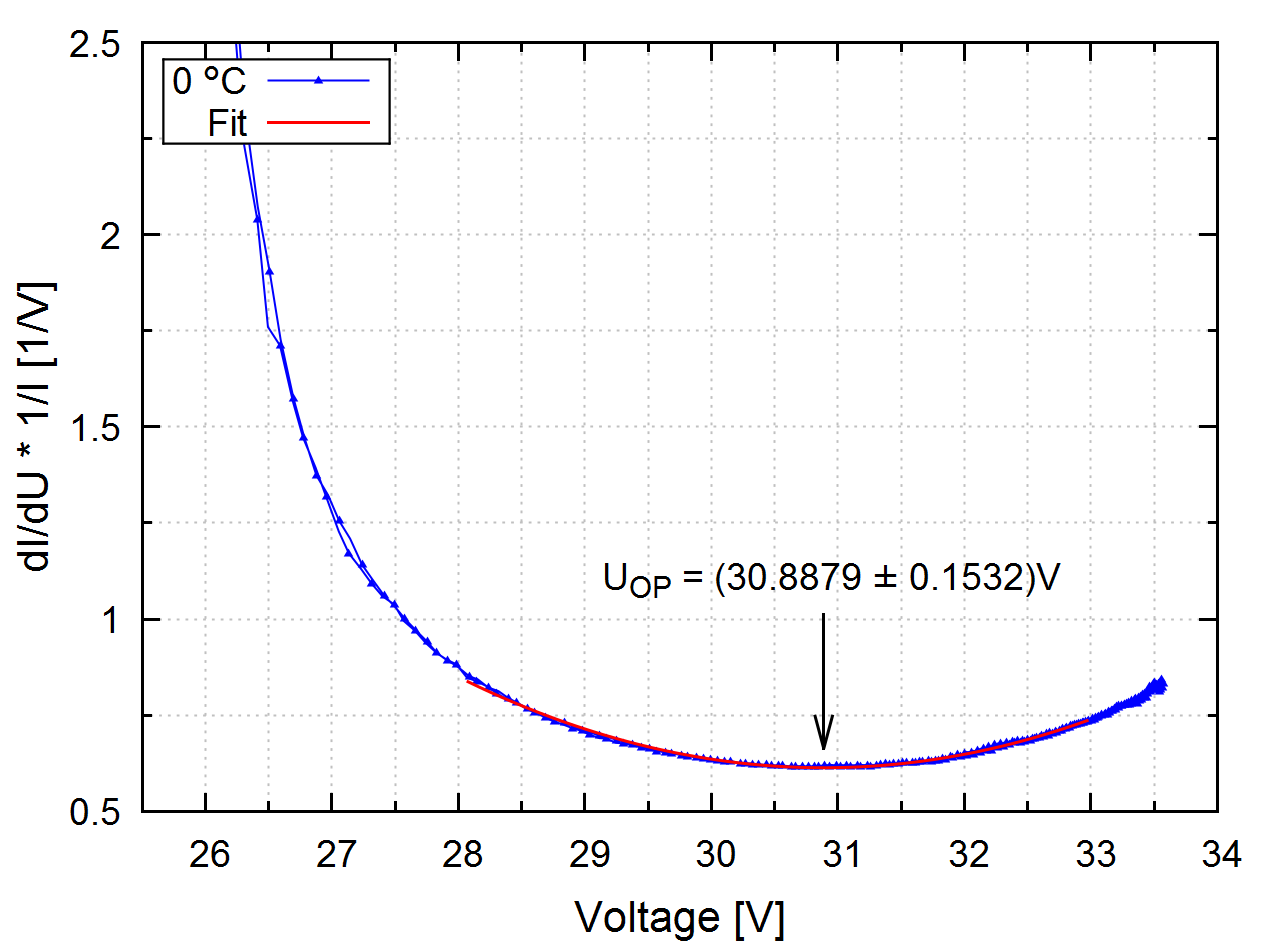
\includegraphics[width=0.49\textwidth]{./plots/iu_curve/4x1n6_op_0.png}}
	\hfill
	\subfloat[(s)-configuration $\SI{-25}{\degreeCelsius}$] {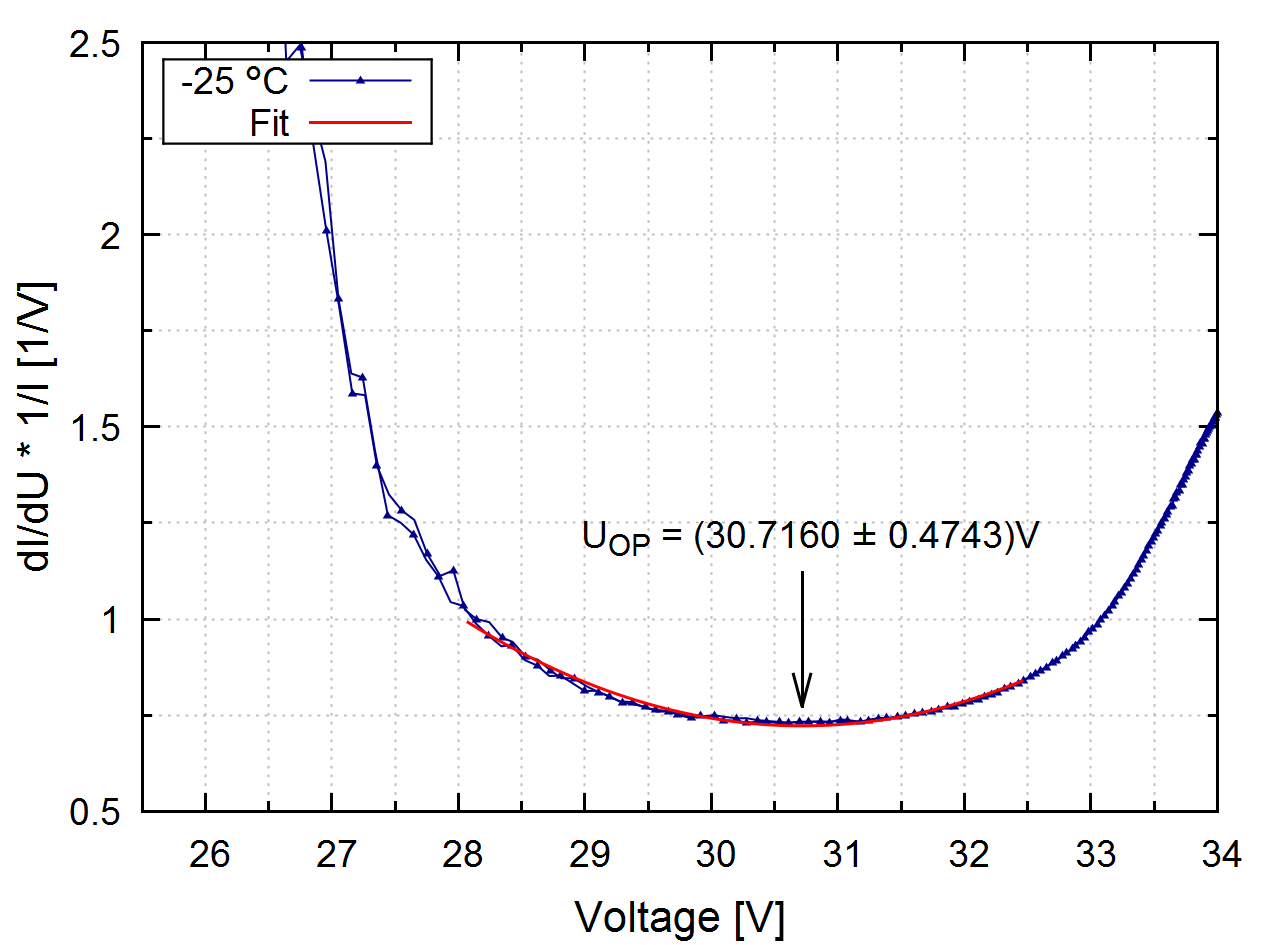
\includegraphics[width=0.38\textwidth]{./plots/iu_curve/4x1n6_op_-25.png}}
	\hfill
	\caption[Operation voltage fits (hyrbid)]{Fits for determining the operation voltage of a hybrid board. }
	\label{ap:B:optimal_fits_hybrid}
\end{figure}

\newpage

\section{Derivation methodology} \label{ap:B:sec:derivation}

For deriving a set of data consisting $x$ and $y$ values with $y(x)$, a linear regression algorithm has been implemented in \texttt{C++}. It fits a linear function 
\begin{align*}
y(x)=m\cdot x+y_0 
\end{align*}
to a number $n$ of data points where the data point lies right in the middle of the interval, so $\frac{n-1}{2}$ data points before and after will be included. This necessitates $n$ to be odd and $>3$.

\section{Energy spectra} \label{ap:energy_spectra}

The data of the fits for the energy spectra of the LYSO crystal is given in table \ref{ap:B:tab:energy_spectra}, more detailed plots can be seen in figure \ref{ap:B:energy_spectra1}. 

% Table generated by Excel2LaTeX from sheet 'Tabelle1'
\begin{table}[H]
	\small
	\centering
	\makebox[\textwidth]{
	\begin{tabular}{c|ccccc}
		\toprule[2pt]
		Source & Energy [$\si{\keV}$] & $\mu$ & $\sigma$ & FWHM [$\si{\keV}$] & $R$ [\%] \\
		\midrule
		& \multicolumn{5}{c}{$T=\SI{25}{\degreeCelsius}$} \\
		\eu{} & 121.80 & 321.92 $\pm$ 1.57  & 35.74 $\pm$ 7.56  & 22.62 $\pm$ 4.78  & 18.57 $\pm$ 3.93 \\
		\eu{} & 344.00 & 1238.11 $\pm$ 1.74  & 172.53 $\pm$ 17.16 & 109.20 $\pm$ 10.86 & 31.74 $\pm$ 3.16 \\
		\ba{} & 356.00 & 1260.24 $\pm$ 0.46  & 234.40 $\pm$ 1.38  & 148.35 $\pm$ 0.87  & 41.67 $\pm$ 0.25 \\
		\na{} ($e^+$) & 511.00 & 2085.84 $\pm$ 1.01 & 204.30 $\pm$ 3.53  & 129.30 $\pm$ 2.23  & 25.30 $\pm$ 0.44 \\
		\cs{} & 661.60 & 2373.58 $\pm$ 0.49  & 219.77 $\pm$ 2.64  & 139.09 $\pm$ 1.67  & 21.02 $\pm$ 0.25 \\
		\na{}  & 1274.50 & 4736.84 $\pm$ 6.01  & 399.79 $\pm$ 869.50 & 253.03 $\pm$ 550.32 & 19.85 $\pm$ 43.18 \\
		\co{} & 1252.90 & 4512.80 $\pm$ 5.67  & 516.36 $\pm$ 11.55 & 326.81 $\pm$ 7.31  & 26.08 $\pm$ 0.58 \\ 
		 & \multicolumn{5}{c}{$T=\SI{-25}{\degreeCelsius}$} \\
		\eu{} & 121.80 & 348.85 $\pm$ 0.46  & 55.21 $\pm$ 6.98  & 33.64 $\pm$ 4.25  & 27.62 $\pm$ 3.49 \\
		\eu{} & 244.70 & 883.46 $\pm$ 7.48  & 154.32 $\pm$ 794.50 & 94.03 $\pm$ 484.09 & 38.43 $\pm$ 197.83 \\
		\eu{} & 344.00 & 1379.17 $\pm$ 1.21  & 124.19 $\pm$ 6.15  & 75.67 $\pm$ 3.75  & 22.00 $\pm$ 1.09 \\
		\ba{} & 356.00 & 1230.25 $\pm$ 0.45  & 195.05 $\pm$ 1.18  & 118.84 $\pm$ 0.72  & 33.38 $\pm$ 0.20 \\
		\na{} ($e^+$) & 511.00 & 2111.80 $\pm$ 0.76 & 177.61 $\pm$ 1.93  & 108.22 $\pm$ 1.18  & 21.18 $\pm$ 0.23 \\
		\cs{} & 661.60 & 2189.56 $\pm$ 0.49  & 201.51 $\pm$ 4.79  & 122.78 $\pm$ 2.92  & 18.56 $\pm$ 0.44 \\
		60Co  & 1173.20 & 4132.47 $\pm$ 25.52 & 240.11 $\pm$ 92.17 & 146.30 $\pm$ 56.16 & 12.47 $\pm$ 4.79 \\
		\co{} & 1274.50 & 5011.38 $\pm$ 3.26  & 357.95 $\pm$ 8.16  & 218.10 $\pm$ 4.97  & 17.11 $\pm$ 0.39 \\
		\co{} & 1252.90 & 5111.35 $\pm$ 4.96  & 1096.87 $\pm$ 316.93 & 668.32 $\pm$ 193.10 & 53.34 $\pm$ 15.41 \\
		\bottomrule[2pt]
	\end{tabular}%
	}
	\caption{Fits for the energy spectra.}
	\label{ap:B:tab:energy_spectra}%
\end{table}%

\newpage

\begin{figure}[h]
	\subfloat[\eu{} energy calibration spectrum for $\SI{25}{\degreeCelsius}$] {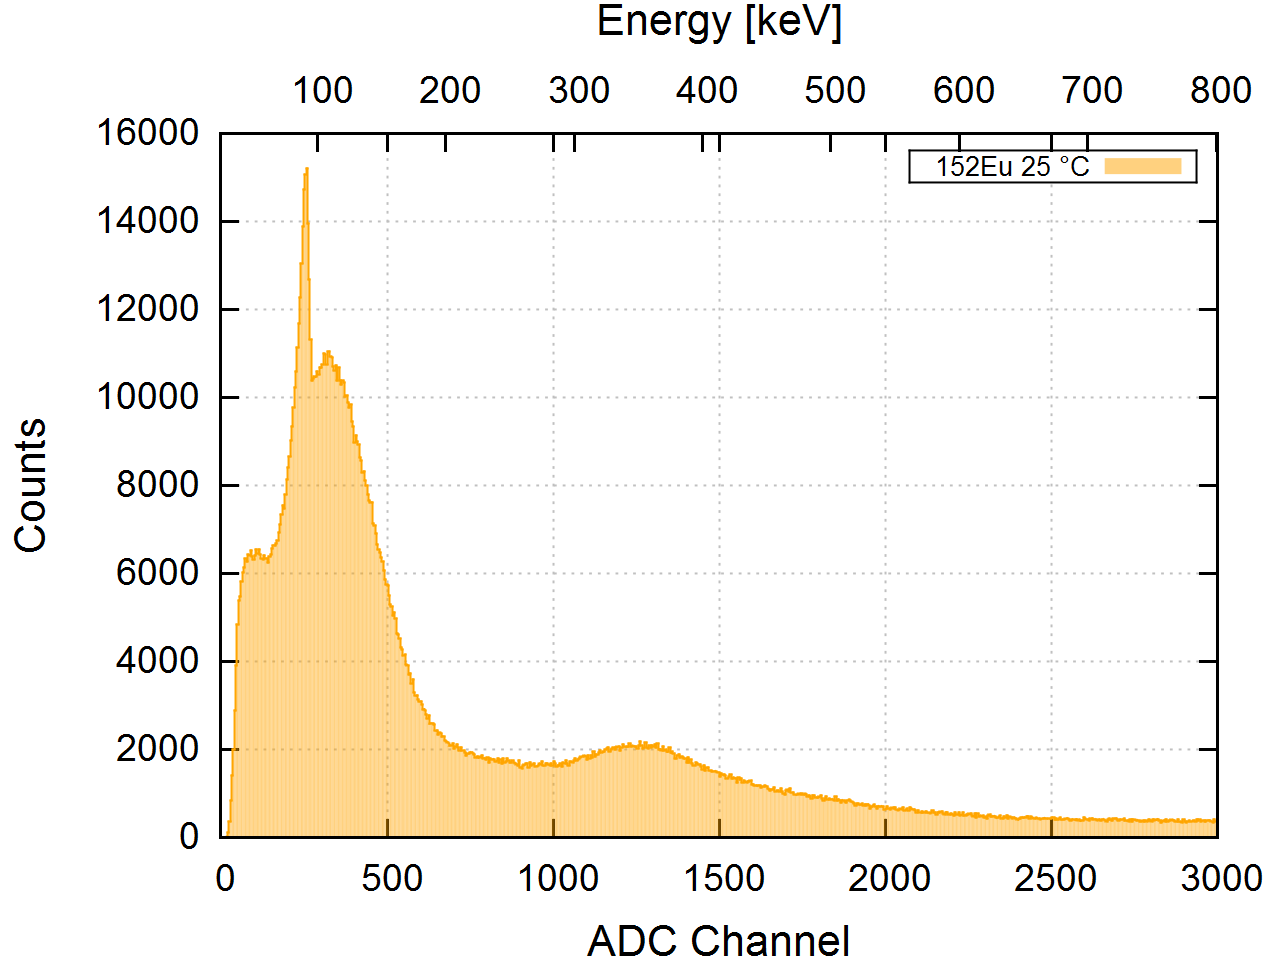
\includegraphics[width=0.49\textwidth]{./plots/energy/lyso_eu25.png}}
	\hfill
	\subfloat[\eu{} energy calibration spectrum for $\SI{-25}{\degreeCelsius}$] {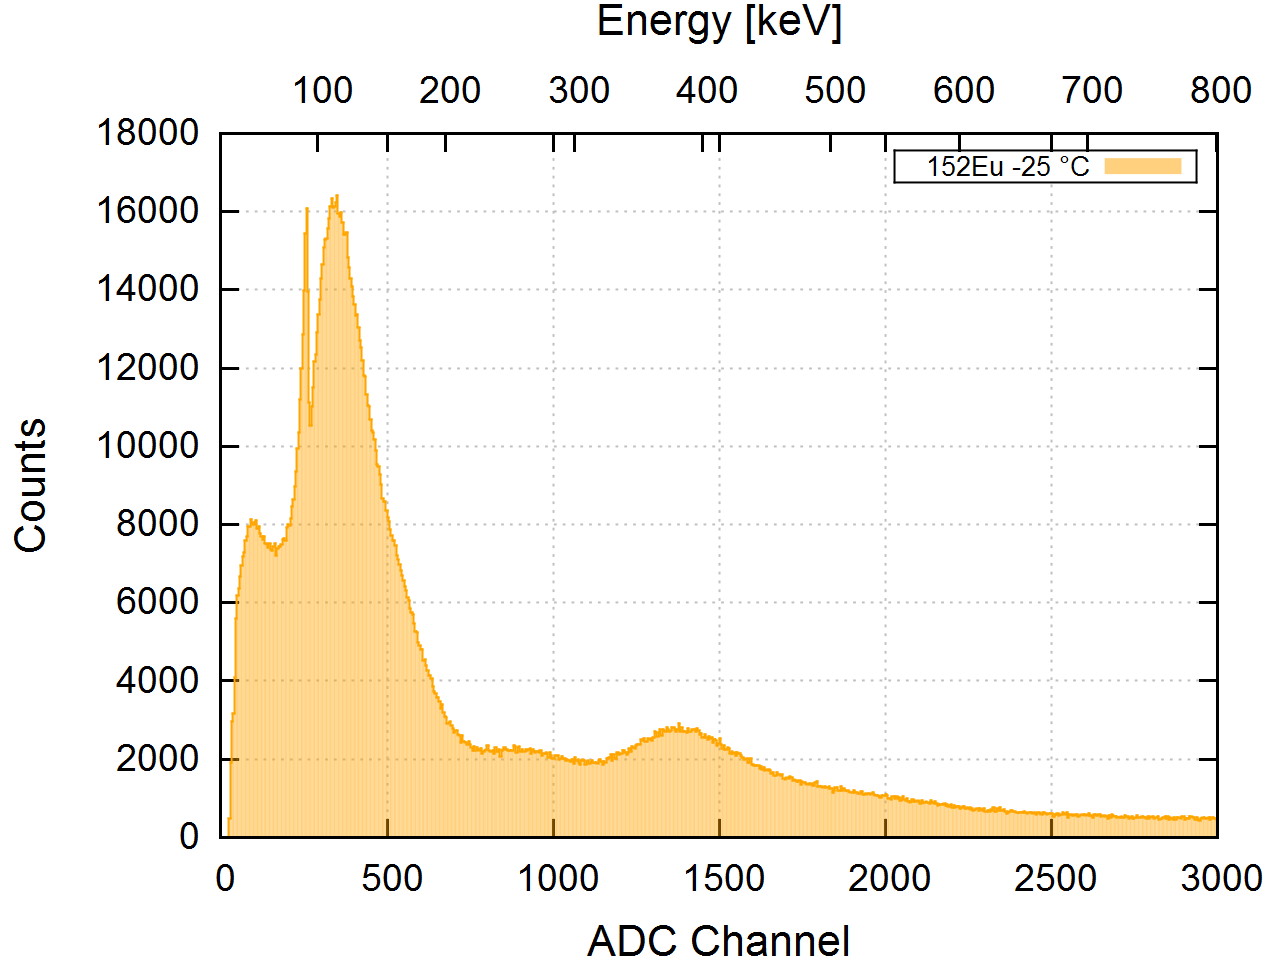
\includegraphics[width=0.49\textwidth]{./plots/energy/lyso_eu-25.png}}
	\hfill
	\subfloat[\ba{} energy calibration spectrum for $\SI{25}{\degreeCelsius}$] {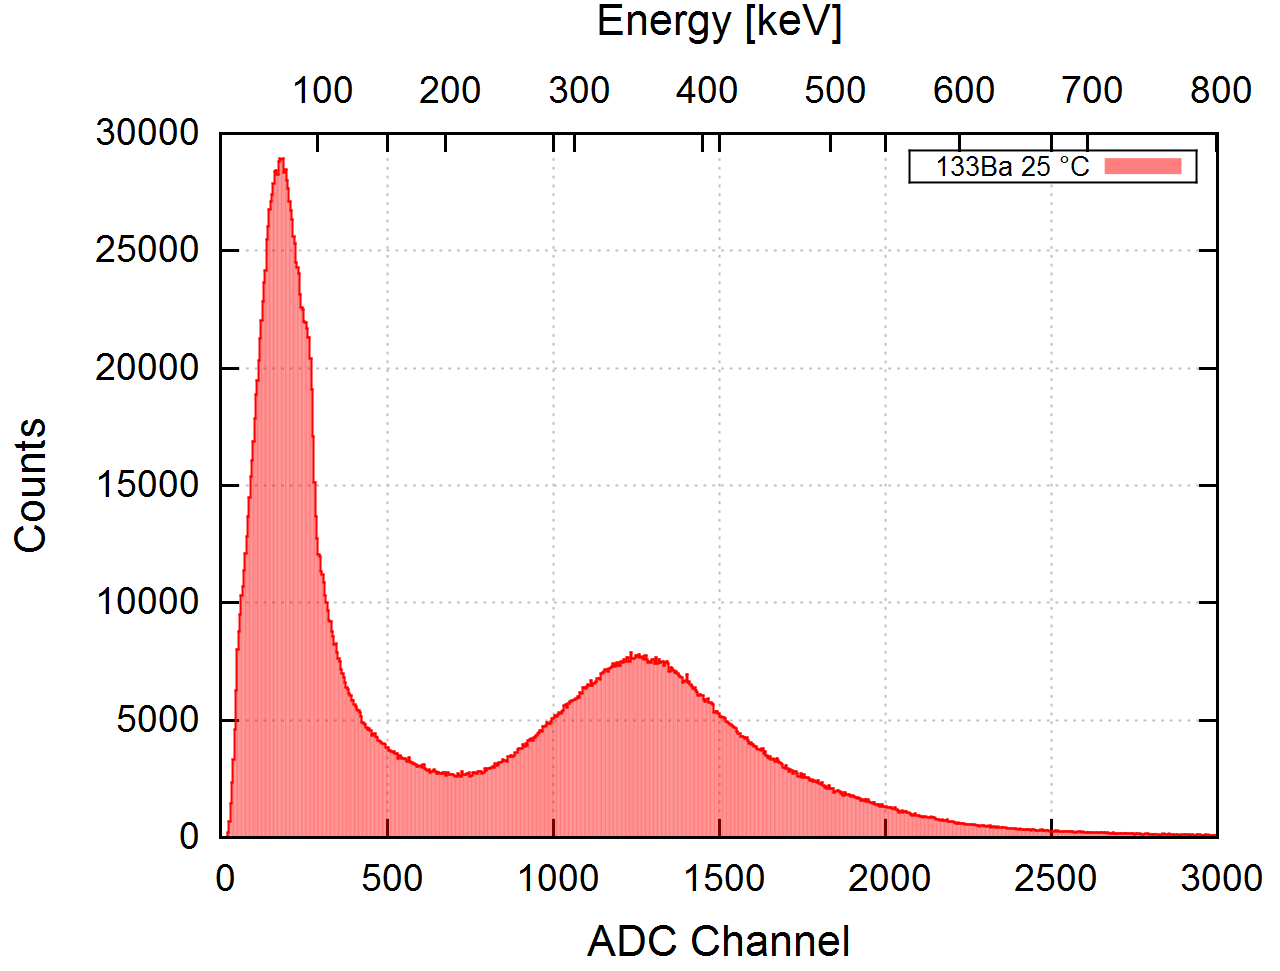
\includegraphics[width=0.49\textwidth]{./plots/energy/lyso_ba25.png}}
	\hfill
	\subfloat[\ba{} energy calibration spectrum for $\SI{-25}{\degreeCelsius}$] {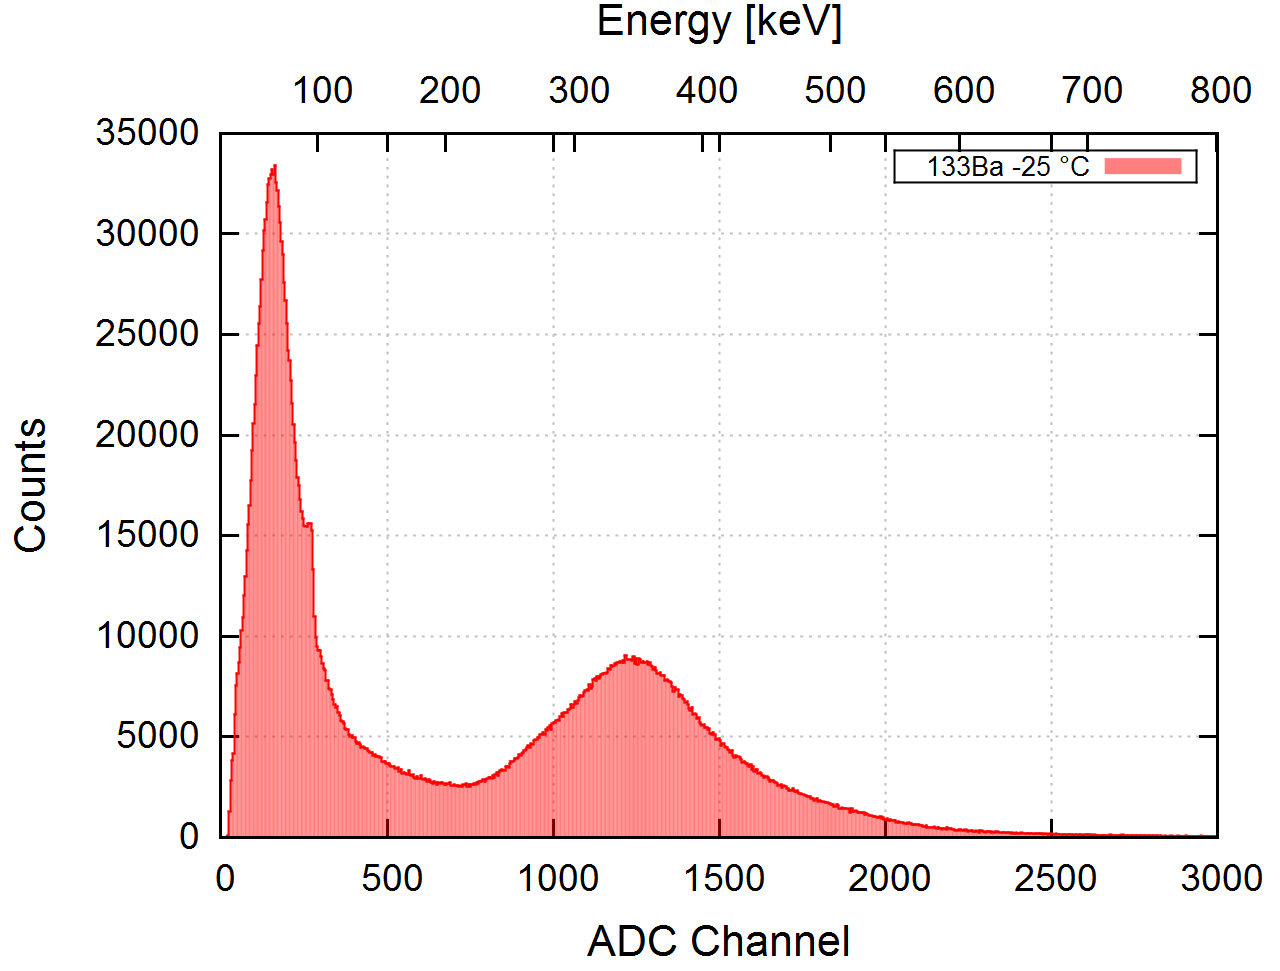
\includegraphics[width=0.49\textwidth]{./plots/energy/lyso_ba-25.png}}
	\hfill
	\subfloat[\co{} energy calibration spectrum for $\SI{25}{\degreeCelsius}$] {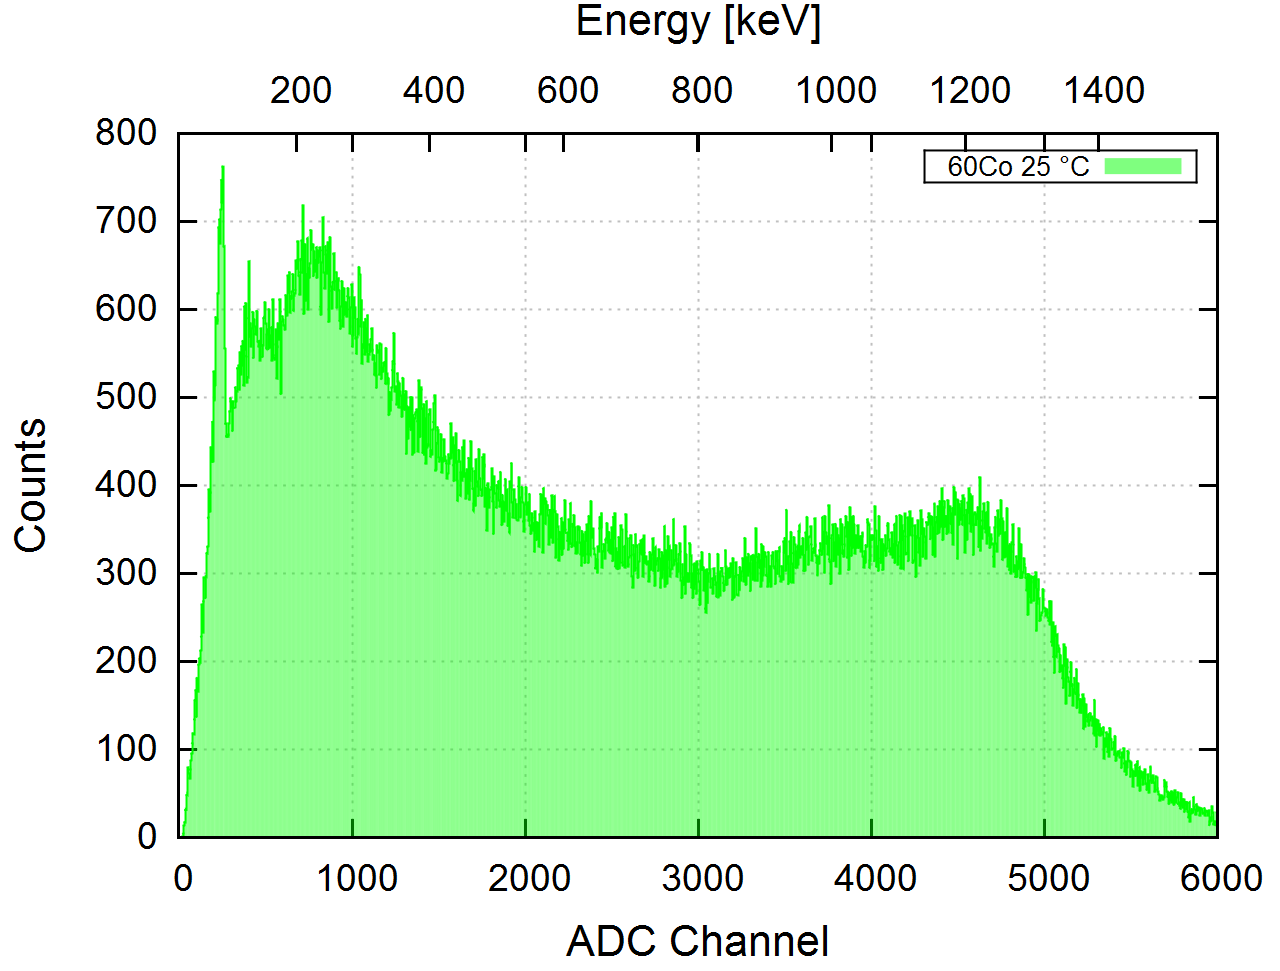
\includegraphics[width=0.49\textwidth]{./plots/energy/lyso_co25.png}}
	\hfill
	\subfloat[\co{} energy calibration spectrum for $\SI{-25}{\degreeCelsius}$] {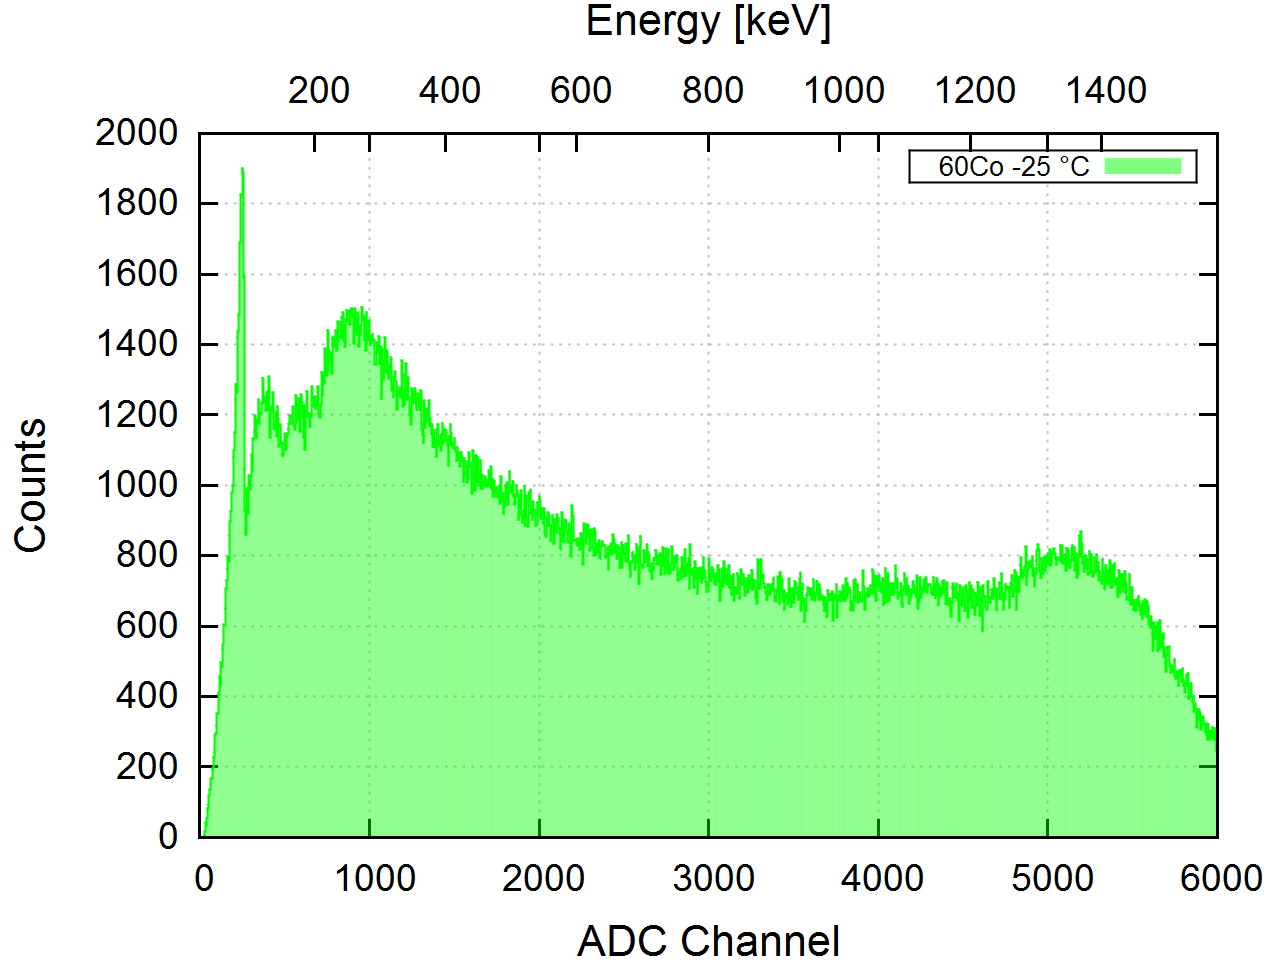
\includegraphics[width=0.49\textwidth]{./plots/energy/lyso_co-25.png}}
	\hfill
	\caption[LYSO energy calibration spectra (detailed)]{Higher resolution energy calibration spectra. Continuation on next page. }
	\label{ap:B:energy_spectra1}
\end{figure}



\begin{figure}[h]
	\ContinuedFloat
	\subfloat[\cs{} energy calibration spectrum for $\SI{25}{\degreeCelsius}$] {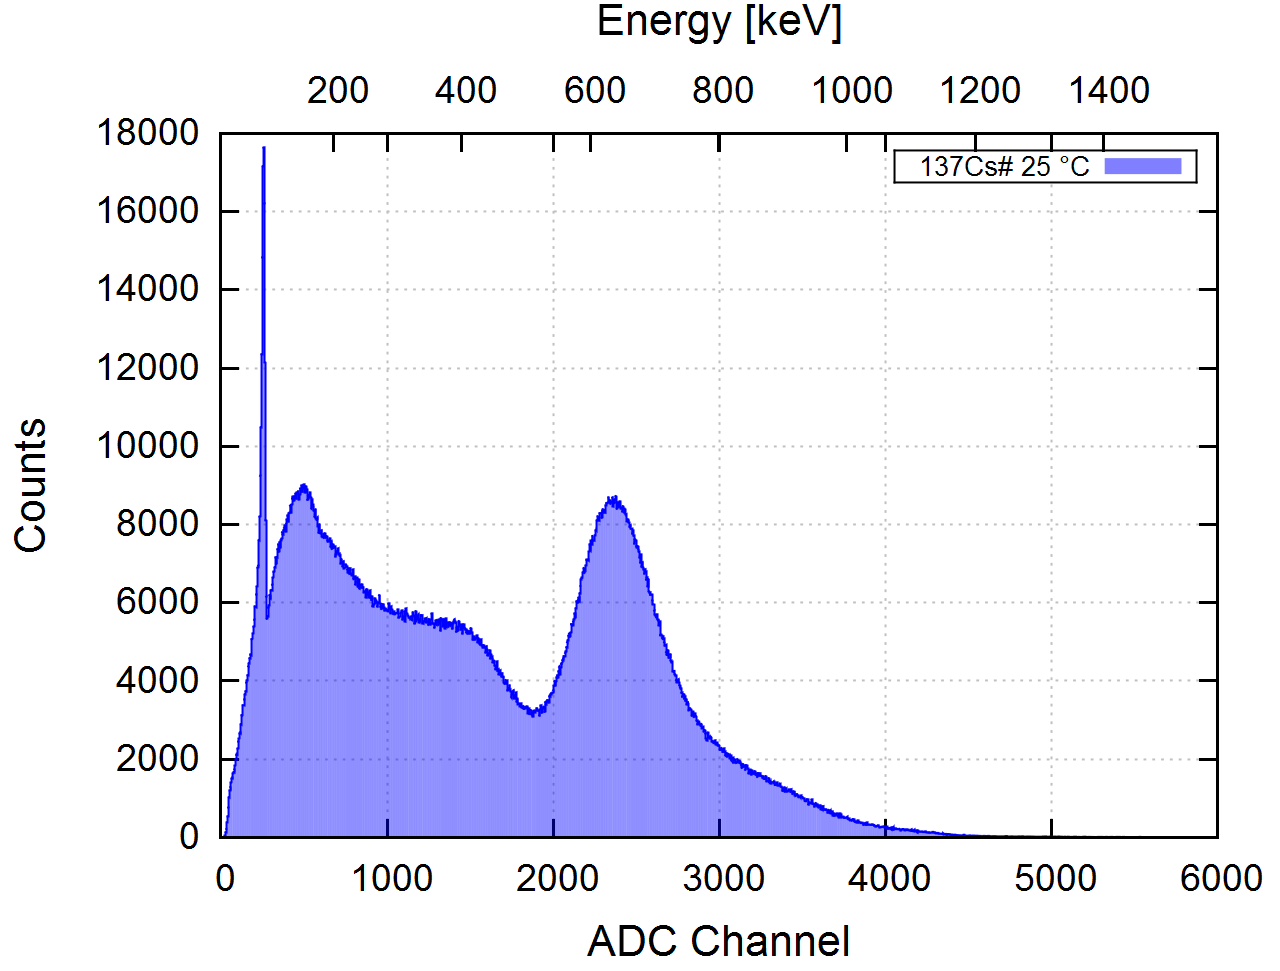
\includegraphics[width=0.49\textwidth]{./plots/energy/lyso_cs25.png}}
	\hfill
	\subfloat[\cs{} energy calibration spectrum for $\SI{-25}{\degreeCelsius}$] {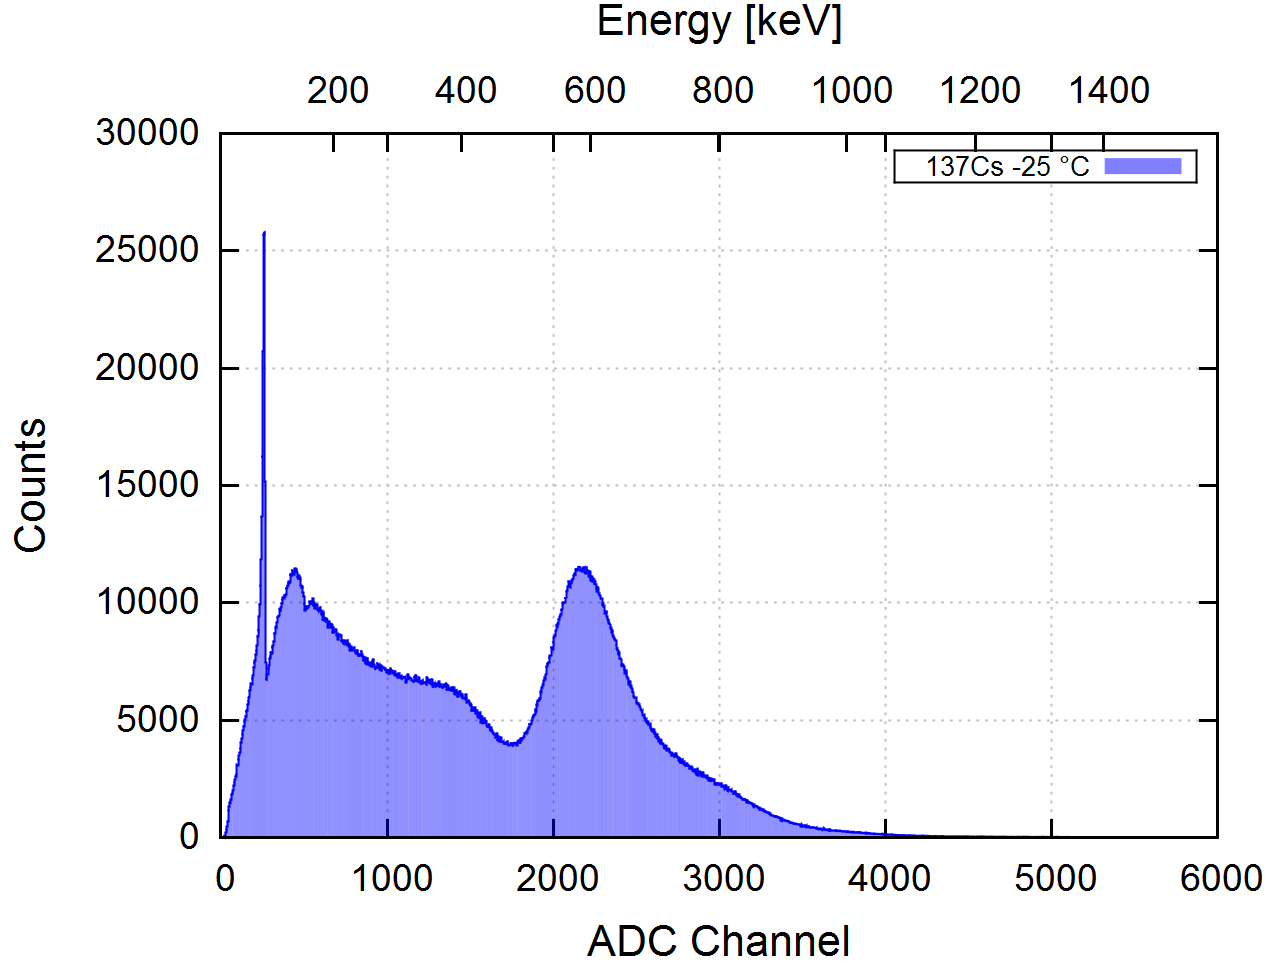
\includegraphics[width=0.49\textwidth]{./plots/energy/lyso_cs-25.png}}
	\hfill
	\subfloat[\na{} energy calibration spectrum for $\SI{25}{\degreeCelsius}$] {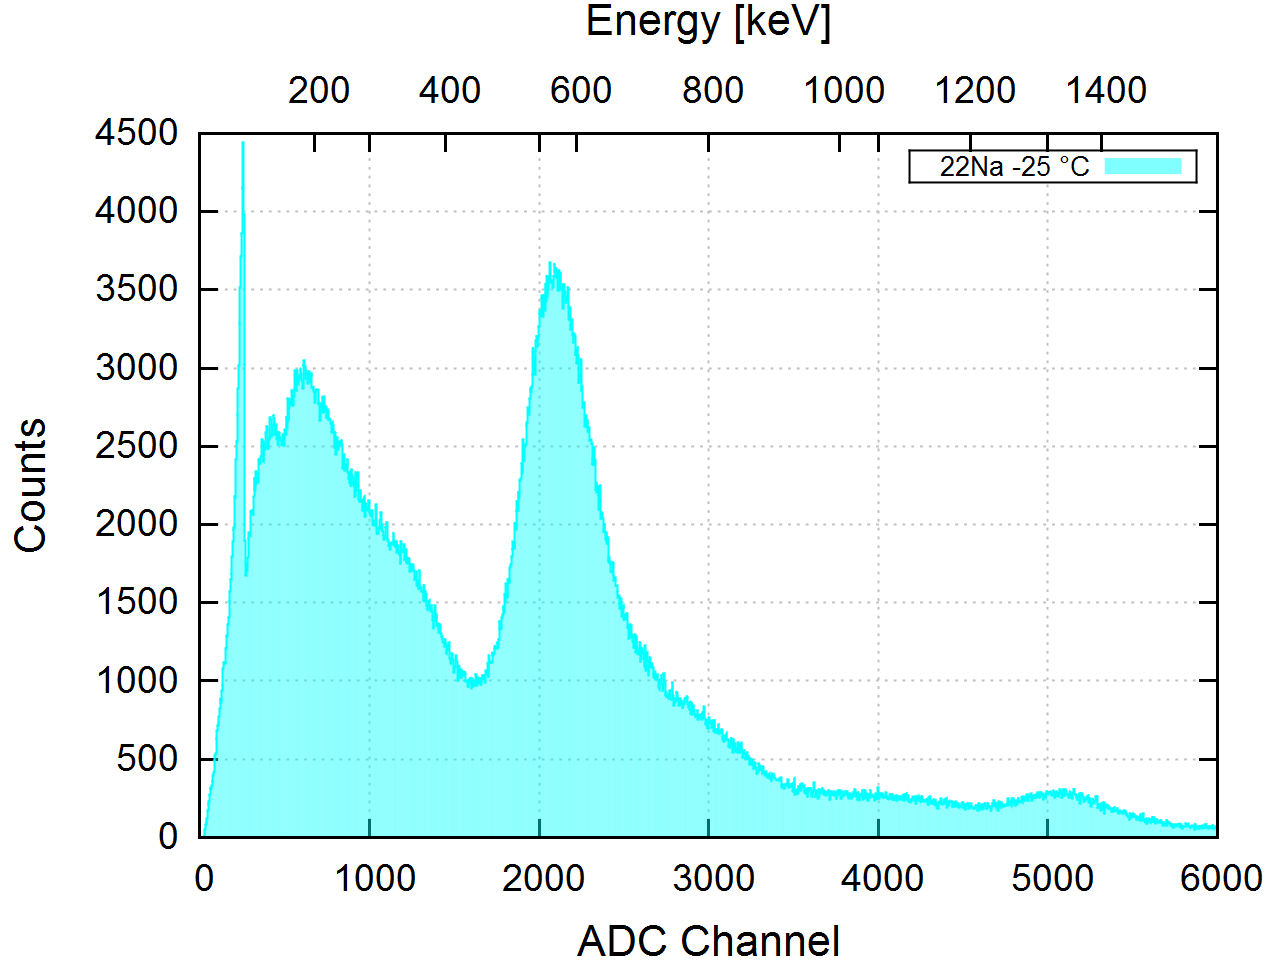
\includegraphics[width=0.49\textwidth]{./plots/energy/lyso_na-25.png}}
	\hfill
	\subfloat[\na{} energy calibration spectrum for $\SI{-25}{\degreeCelsius}$] {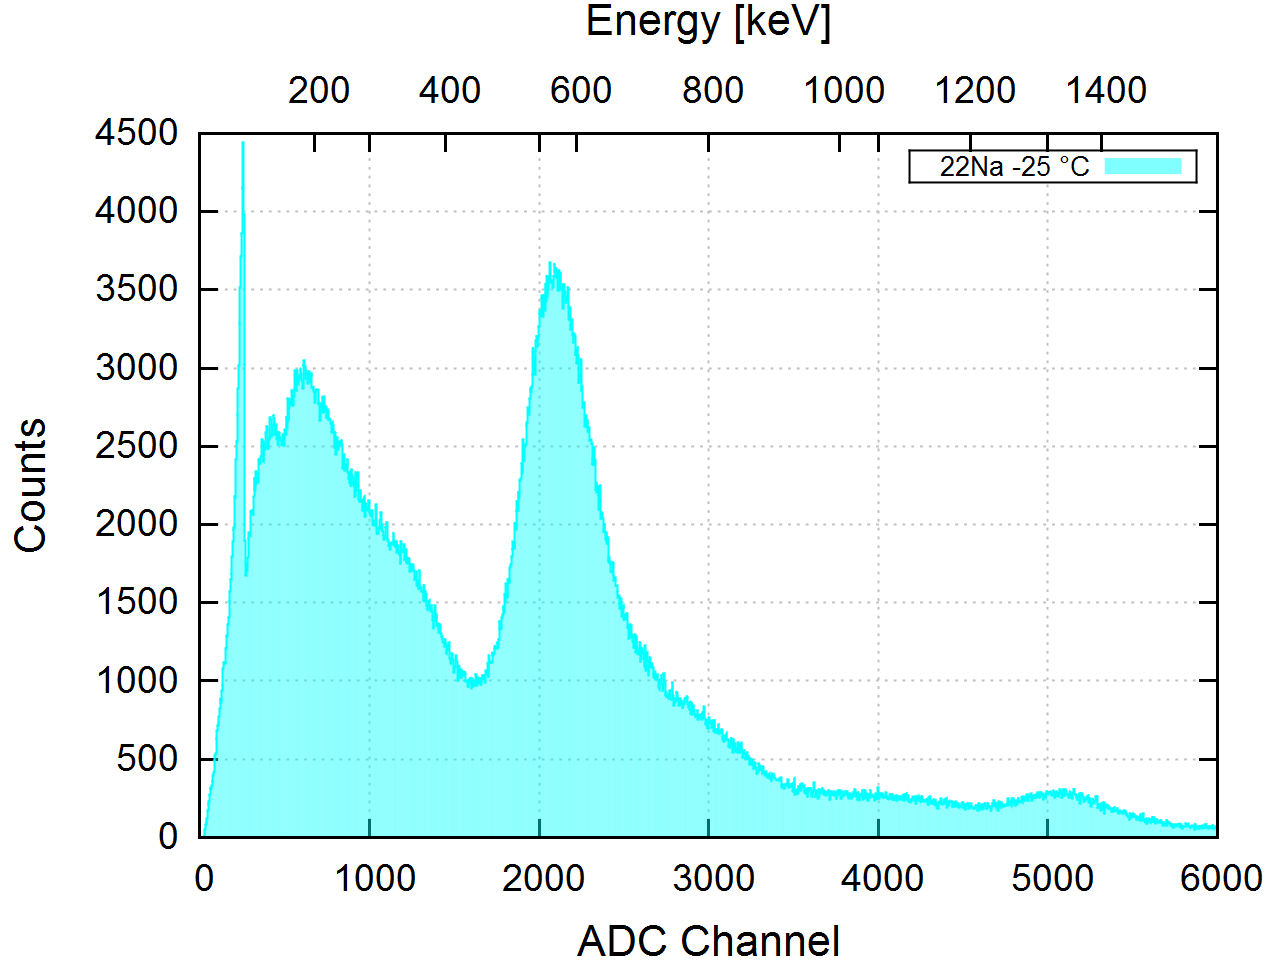
\includegraphics[width=0.49\textwidth]{./plots/energy/lyso_na-25.png}}
	\hfill
	\caption*{Higher resolution energy calibration spectra. Continuation from prior page.}
	\label{ap:B:energy_spectra2}
\end{figure}

\newpage

\chapter{Pictures and schematics}\label{ap:C:pictures}

\begin{figure}[h]
	\subfloat[Single SiPM with partially molten epoxy entrance window] {\includegraphics[width=0.40 \textwidth]{./pictures/SiPM_microscope/1x1n5_SiPM_damaged.jpg}}
	\hfill
	\subfloat[$50\si{\micro\meter}\times 50\si{\micro\meter}$ sized microcells ] {\includegraphics[width=0.55\textwidth]{./pictures/SiPM_microscope/SiPM_zoomed_small.jpg}}
	\hfill
	\caption[SiPM under light microscope]{Zoomed photograph of a SiPM with a light microscope\footnote{Thanks to I. Physikalische Institut for accessing the device}. Note the damage of the epoxy entrance window due to soldering with a soldering bolt. After some issues, soldering was done with a hot plate and solder paste.}
	\label{ap:C:SiPM_microscope}
\end{figure}

\begin{figure}[H]
	\subfloat[Different SiPM configurations] {\includegraphics[width=0.49 \textwidth]{./pictures/Plastic/SiPM.jpg}}
	\hfill
	\subfloat[SiPM masks] {\includegraphics[width=0.49\textwidth]{./pictures/Plastic/SiPM_mask.jpg}}
	\hfill
	\caption[SiPM with masks]{Photograph of differently equipped SiPM-boards and masks to fill the spacing between board and scintillator material. Note the attached reflective foil .}
	\label{ap:C:SiPM_masks}
\end{figure}

\newpage

\begin{figure}[h]
	\subfloat[Plastic scintillator \tit{EJ-248M} from \tit{ELJEN} with a thickness of $\SI{10}{\milli\meter}$] {\includegraphics[width=0.49 \textwidth]{./pictures/Plastic/plastic.jpg}}
	\hfill
	\subfloat[Various inorganic scintillators, BGO and \baf{} already wrapped in teflon foil and black tape ] {\includegraphics[width=0.49\textwidth]{./pictures/Plastic/inorganics.jpg}}
	\hfill
	\caption[Various scintillators]{Photograph of scintillators. The plastic scintillator is in the shape of the measurement setup in chapter 4. For the energy measurements, the LYSO and the PWO crystals were used.}
	\label{ap:C:scintillators}
\end{figure}

\begin{figure}[H]
	\subfloat[Different SiPM types.] {\includegraphics[width=0.49 \textwidth]{./pictures/SiPMs/unterschiedlice_SiPM.JPG}}
	\hfill
	\subfloat[Unequipped front of back of the SiPM-boards] {\includegraphics[width=0.49\textwidth]{./pictures/SiPMs/boards.JPG}}
	\hfill
	\caption[Various SiPM types]{Photograph of four different SiPM types and the SiPM-board. From left to right: large SiPM with $\SI{6}{\milli\meter}\times\SI{6}{\milli\meter}$ active area and $\SI{50}{\micro\meter}$ pixel size, the SiPM type used for this thesis with $\SI{3}{\milli\meter}\times\SI{3}{\milli\meter}$ active area and $\SI{50}{\micro\meter}$ pixel size, a small SiPM with $\SI{1}{\milli\meter}\times\SI{1}{\milli\meter}$ active area and $\SI{50}{\micro\meter}$ pixel size and a new SiPM package type (KETEK WB series) with $\SI{3}{\milli\meter}\times\SI{3}{\milli\meter}$ active area and $\SI{15}{\micro\meter}$ pixel size and a thickness of $\SI{0.6}{\milli\meter}$ (!). The second picture shows the unequipped front and back of the SiPM-boards which were designed for the $\SI{3}{\milli\meter}\times\SI{3}{\milli\meter}$ KETEK EB series. }
	\label{ap:C:Siverse_SiPMs}
\end{figure}

\newpage

\begin{figure}[H]
	\centering
	\includegraphics[width=1\textwidth]{./graphics/ch5/plastic.png}
	\caption[Schematic of the plastic scintillator]{Schematic of the plastic scintillator. Dimensioning in $\si{\milli\meter}$. The SiPM positions are marked in red.}    
	\label{ap:C:plastic}
\end{figure}

\begin{figure}[H]
	\subfloat[Schematic of the LYSO crystal] {\includegraphics[width=0.49 \textwidth]{./graphics/ch5/LYSO.png}}
	\hfill
	\subfloat[Schematic of the \pwo{} crystal] {\includegraphics[width=0.49\textwidth]{./graphics/ch5/PWO.png}}
	\hfill
	\caption[Schematics of the used scintillators]{Schematic of the used scintillators. Dimensioning in $\si{\milli\meter}$. The SiPM positions are marked in red.}
	\label{ap:C:crystals}
\end{figure}
















